% Gabarit pandoc des corrigés publiés (brut et guidé). Contenu sans marque ni nom de site.
% Compilation : lualatex (latexmk -lualatex).
% Le Markdown reste la source unique : ne pas éditer ce fichier .tex à la main.
\documentclass[11pt,a4paper]{article}

% --- Moteur, polices (Latin Modern) et langue ---------------------------------
\usepackage{iftex}
\ifLuaTeX\else\errmessage{Ce document se compile avec lualatex}\fi
\usepackage{amsmath,amssymb,mathtools}
\usepackage{fontspec}
% mathrm=sym : \mathrm prend ses glyphes dans la police mathématique (ℓ, μ, Ω), comme KaTeX.
\usepackage[math-style=TeX,bold-style=TeX,mathrm=sym]{unicode-math}
% Repli pour les glyphes absents de Latin Modern (indices et exposants Unicode,
% flèches, filets des schémas en texte, symboles) : DejaVu, puis Latin Modern Math
% (ℓ, lettres mathématiques Unicode des légendes).
\directlua{
  luaotfload.add_fallback("repliTexte", {"DejaVuSerif:mode=harf;", "DejaVuSans:mode=harf;", "file:latinmodern-math.otf:mode=harf;"})
  luaotfload.add_fallback("repliMono", {"DejaVuSansMono:mode=harf;", "DejaVuSans:mode=harf;", "file:latinmodern-math.otf:mode=harf;"})
}
\setmainfont{Latin Modern Roman}[RawFeature={fallback=repliTexte}]
\setsansfont{Latin Modern Sans}[RawFeature={fallback=repliTexte}]
\setmonofont{Latin Modern Mono}[RawFeature={fallback=repliMono}]
\setmathfont{Latin Modern Math}
\usepackage[french]{babel}
\frenchsetup{SmallCapsFigTabCaptions=false}

% --- Mise en page --------------------------------------------------------------
\usepackage[a4paper,margin=2.2cm,headheight=14pt,footskip=1.2cm]{geometry}
\usepackage{microtype}
\setlength{\emergencystretch}{4em}
\tolerance=1500
\setlength{\parindent}{0pt}
\setlength{\parskip}{0.55\baselineskip plus 2pt minus 1pt}
\usepackage{xcolor}
% Gris nommés : babel-french rend « ! » actif dans le document.
\definecolor{gris2}{gray}{0.98}
\definecolor{gris3}{gray}{0.97}
\definecolor{gris5}{gray}{0.95}
\definecolor{gris35}{gray}{0.65}
\definecolor{gris40}{gray}{0.60}
\definecolor{gris45}{gray}{0.55}
\definecolor{gris50}{gray}{0.50}
\definecolor{gris55}{gray}{0.45}
\definecolor{gris60}{gray}{0.40}
\definecolor{gris65}{gray}{0.35}
\definecolor{gris70}{gray}{0.30}
\definecolor{gris80}{gray}{0.20}
\definecolor{gris85}{gray}{0.15}
\usepackage{graphicx}
\usepackage{float}
\usepackage{caption}
\captionsetup{font=small,labelformat=empty,justification=centering}
\usepackage{booktabs,longtable,array,multirow,calc}
\usepackage{siunitx}
\sisetup{locale=FR}
\usepackage[version=4]{mhchem}
\usepackage{listings}
\usepackage{fancyhdr}
\usepackage{lastpage}
\usepackage[most]{tcolorbox}
\usepackage{enumitem}
\setlist{nosep,leftmargin=*,topsep=2pt}
\usepackage[hidelinks,unicode]{hyperref}
\usepackage{bookmark}
\hypersetup{pdftitle={X MP — Physique et SI 2026},pdfauthor={Rédigé par IA},pdfcreator={LaTeX},pdfsubject={Corrigé guidé}}
\usepackage{xurl}

% --- Pandoc : listes, tableaux, figures ----------------------------------------
\providecommand{\passthrough}[1]{#1}
\providecommand{\tightlist}{\setlength{\itemsep}{0pt}\setlength{\parskip}{0pt}}

\makeatletter
\def\maxwidth{\ifdim\Gin@nat@width>\linewidth\linewidth\else\Gin@nat@width\fi}
\def\maxheight{\ifdim\Gin@nat@height>0.55\textheight 0.55\textheight\else\Gin@nat@height\fi}
\makeatother
\setkeys{Gin}{width=\maxwidth,height=\maxheight,keepaspectratio}
\setcounter{secnumdepth}{-\maxdimen}
\providecommand{\pandocbounded}[1]{#1}
\usepackage{longtable,booktabs,array}

% --- Code (listings) -----------------------------------------------------------
\lstset{
  basicstyle=\ttfamily\small,
  columns=fullflexible,
  keepspaces=true,
  breaklines=true,
  breakatwhitespace=false,
  postbreak=\mbox{\textcolor{gris50}{$\hookrightarrow$}\space},
  frame=single,
  rulecolor=\color{gris35},
  framesep=4pt,
  xleftmargin=5pt,xrightmargin=5pt,
  backgroundcolor=\color{gris3},
  keywordstyle=\bfseries,
  commentstyle=\color{gris65},
  stringstyle=\color{gris80},
  showstringspaces=false,
  tabsize=4,
  extendedchars=true,
  aboveskip=6pt,belowskip=6pt,
}

% --- Macros des corrigés (KaTeX ↔ LaTeX) ---------------------------------------
% Les corrigés sont écrits pour KaTeX : on définit ici ce que KaTeX connaît et
% que LaTeX n'a pas, sans jamais retoucher le Markdown.
\providecommand{\R}{\mathbb{R}}
\providecommand{\N}{\mathbb{N}}
\providecommand{\Z}{\mathbb{Z}}
\providecommand{\Q}{\mathbb{Q}}
\providecommand{\C}{\mathbb{C}}
\providecommand{\dd}{\mathrm{d}}
\providecommand{\llbracket}{\lBrack}
\providecommand{\rrbracket}{\rBrack}
\providecommand{\lBrace}{\lbrace}
\providecommand{\rBrace}{\rbrace}
\providecommand{\Box}{\square}
\providecommand{\Diamond}{\lozenge}
\providecommand{\varnothing}{\emptyset}
\providecommand{\argmax}{\operatorname*{arg\,max}}
\providecommand{\argmin}{\operatorname*{arg\,min}}
\renewcommand{\leq}{\leqslant}
\renewcommand{\geq}{\geqslant}

% Équation hors texte : réduite à la largeur de la ligne si elle déborde.
\newsavebox{\boiteequation}
\newcommand{\equationajustee}[1]{%
  \sbox{\boiteequation}{$\displaystyle #1$}%
  \ifdim\wd\boiteequation>\linewidth
    \[\resizebox{\linewidth}{!}{\usebox{\boiteequation}}\]%
  \else
    \[#1\]%
  \fi}

% --- Encadrés pédagogiques (sobres, lisibles en noir et blanc) -----------------
\tcbset{
  encadre/.style={
    enhanced,breakable,sharp corners,
    colback=white,colframe=gris55,
    boxrule=0.4pt,leftrule=2.2pt,
    left=6pt,right=6pt,top=3pt,bottom=3pt,
    before skip=6pt,after skip=6pt,
    fonttitle=\bfseries\small,coltitle=black,
    attach title to upper,after title={\quad},
    parbox=false,
  }
}
\newtcolorbox{indication}[1]{encadre,colframe=gris45,colback=gris2,title={Indication~#1}}
\newtcolorbox{methode}{encadre,colframe=gris70,title={Méthode}}
\newtcolorbox{piege}{encadre,colframe=gris85,boxrule=0.8pt,leftrule=2.2pt,title={Piège}}
\newtcolorbox{jury}{encadre,colframe=gris60,colback=gris5,title={Jury}}
\newtcolorbox{encadrenote}{encadre,colframe=gris40}

% --- Titres de section ---------------------------------------------------------
\usepackage{titlesec}
\titleformat{\section}{\Large\bfseries}{}{0pt}{}
\titleformat{\subsection}{\large\bfseries}{}{0pt}{}
\titleformat{\subsubsection}{\normalsize\bfseries}{}{0pt}{}
\titlespacing*{\section}{0pt}{14pt plus 4pt minus 2pt}{6pt}
\titlespacing*{\subsection}{0pt}{10pt plus 3pt minus 2pt}{4pt}
\titlespacing*{\subsubsection}{0pt}{8pt plus 2pt minus 2pt}{2pt}

% --- En-tête et pied de page ---------------------------------------------------
\pagestyle{fancy}
\fancyhf{}
\fancyhead[L]{\small\textsc{Corrigé guidé} · X MP}
\fancyhead[R]{\small Physique et SI 2026}
\fancyfoot[L]{\footnotesize Corrigé rédigé par IA, non officiel}
\fancyfoot[R]{\footnotesize \thepage\,/\,\pageref*{LastPage}}
\renewcommand{\headrulewidth}{0.4pt}
\renewcommand{\footrulewidth}{0pt}
\fancypagestyle{plain}{\fancyhf{}\fancyfoot[R]{\footnotesize \thepage\,/\,\pageref*{LastPage}}\fancyfoot[L]{\footnotesize Corrigé rédigé par IA, non officiel}\renewcommand{\headrulewidth}{0pt}}

\begin{document}
\thispagestyle{plain}
\begin{center}
  {\small\scshape Corrigé guidé}\par\smallskip
  {\LARGE\bfseries X MP — Physique et SI 2026\par}\medskip
  {\large X · MP · Physique et SI · 2026\par}
\end{center}
\vspace{2pt}\hrule\vspace{8pt}

\emph{Corrigé rédigé par IA, non officiel. Signalez toute erreur.}

\hypertarget{pruxe9sentation-du-sujet}{%
\section{Présentation du sujet}\label{pruxe9sentation-du-sujet}}

\textbf{Cadre.} Cette épreuve de 4 heures est réservée à une partie des candidats MP, les autres composant en Informatique A. La calculatrice est interdite. Les applications numériques se font avec au plus deux chiffres significatifs, et les ordres de grandeur avec un seul. Le sujet compte \textbf{37 questions}, dont beaucoup ont des sous-questions, en deux parties indépendantes. L'énoncé conseille d'y consacrer au plus deux heures chacune. Le fil conducteur est la mission SMILE d'étude du vent solaire.

\textbf{Partie Physique (Q1--Q17).}

\begin{itemize}
\tightlist
\item
  \emph{1. Communications satellite--Terre (Q1--Q5).} C'est un grand classique : propagation d'une onde électromagnétique dans un plasma froid peu dense (l'ionosphère). On écrit le principe fondamental pour une charge, on néglige la force magnétique, puis on obtient la conductivité complexe imaginaire pure et la relation de dispersion \(k^2c^2=\omega^2-\omega_p^2\). Suivent la fréquence plasma, la coupure, les vitesses de phase et de groupe, la dispersion et le choix de la bande Ku.
\item
  \emph{2. Points de Lagrange (Q6--Q17).} On traite le problème restreint des trois corps dans le référentiel tournant : troisième loi de Kepler, forces d'inertie, pseudo-potentiel \(U\), constante de Jacobi et zones d'exclusion, adimensionnement. On calcule ensuite la position de \(\mathrm L_4\) et \(\mathrm L_5\) (triangles équilatéraux) et l'équation de \(\mathrm L_1\) avec son application numérique (1,5 million de km). La partie se termine sur la stabilité : cols de \(U\), rôle stabilisant de la force de Coriolis, linéarisation matricielle, critère de Routh \(27\mu(1-\mu)<1\) et périodes de libration.
\end{itemize}

\textbf{Partie Sciences de l'ingénieur (Q18--Q37).}

\begin{itemize}
\tightlist
\item
  \emph{2.1 Analyse du mécanisme (Q18--Q19).} Graphe de liaisons et schéma cinématique de la chaîne bâti--\allowbreak{}arbre--\allowbreak{}bras--\allowbreak{}panneaux.
\item
  \emph{2.2 Dynamique du déploiement (Q20--Q27).} C'est le cœur calculatoire, pour un système plan bras + panneau à deux pivots et deux ressorts de torsion. On y traite le caractère galiléen du référentiel, la matrice d'inertie d'un parallélépipède, les torseurs d'actions, les vitesses, les accélérations, les torseurs dynamiques, puis deux équations de Lagrange « à la main » par le théorème du moment dynamique.
\item
  \emph{2.3 Validation (Q28--Q30).} Lecture critique de courbes de simulation : blocages en butée, cahier des charges, choc.
\item
  \emph{3. Orientation (Q31--Q37).} Asservissement en position avec boucle de vitesse interne : schéma-bloc, réduction de boucle, précision, classe, correcteur PI.
\end{itemize}

\textbf{Notions mobilisées.} Force de Lorentz, équations de Maxwell en notation complexe, relation de dispersion, paquets d'ondes. Côté mécanique : référentiels non galiléens, énergie, gradient, linéarisation autour d'un équilibre, valeurs propres. Côté SI : cinématique du solide, opérateur d'inertie, torseurs dynamiques et PFD, schémas-blocs, théorème de la valeur finale, classe d'un système. Tout est au programme MP et MP option SI.

\textbf{Difficulté.} La partie 1 de physique est très classique. Le rapport 2026 montre pourtant que les candidats décrochent dès qu'il faut calculer ou interpréter : Q3.b à Q3.d, le commentaire de Q4 et les trois items de Q5 plafonnent entre 27 et 37 \% de réussite. La partie 2 (Q6--Q17) est de loin la plus sélective : seules Q6, Q7.a et Q9 dépassent 30 \% de réussite, et Q10, Q11 et Q14 à Q17 restent sous 10 \%. Elle demande de la rigueur dans les dérivées composées (Q10--Q11) et un peu d'algèbre linéaire (Q15--Q17).

En SI, le bloc dynamique Q21--Q28 est discriminant : hors Q23 et Q24, aucune de ces questions ne dépasse 20 \% de réussite environ, et Q26--Q27 ne sont presque jamais réussies. Un seul signe faux dans une accélération ou un moment de ressort rend inexploitable la forme (54). En automatique, les schémas-blocs (Q31, Q32) passent bien, mais la précision (Q33, environ 12 \%) et l'ordre et la classe de la FTBO (Q35, environ 18 \%) sont peu réussis : ce sont des questions de cours, mais elles demandent un calcul propre.

\textbf{Ce qu'en dit le rapport 2026.} Les pourcentages ci-dessus et dans les encadrés « Jury » sont lus sur les histogrammes du rapport (figures 1a à 2d, p.~2--5) : ce sont des ordres de grandeur. Une question y est « réussie » quand elle a obtenu au moins la moitié des points. Les histogrammes découpent certaines questions en items (« Q4-b », « Q8-a1 »\ldots) et vont jusqu'à « Q38 », alors que le sujet s'arrête à Q37 ; nous rapportons ces items à la numérotation du sujet, sous réserve.

\begin{jury}

Le rapport 2026 (p.~2) note « un très faible taux de réussite à l'échelle globale : 51\% pour la partie I.1, 15\% pour la partie I.2, 30\% pour la partie II.1 et II.2 puis 40\% pour la partie II.3 ». Il rappelle trois exigences (p.~6). Sur les unités : « tout résultat numérique correspondant à une grandeur physique doit impérativement être accompagné de son unité ; en son absence, le résultat ne peut être considéré comme correct. » Sur les sous-questions : « chaque sous-question d'une question numérotée fait l'objet d'une évaluation distincte. » Sur la rédaction : « Une réponse précise, concise, proprement présentée et reposant sur un raisonnement clairement explicité est davantage valorisée que la seule mention d'un résultat, même lorsque celui-ci est correct. »

\end{jury}

\textbf{Questions à ne pas laisser passer.} Q1, Q2, Q3.a--b, Q4, Q6, Q8.a, Q9, Q12, Q16, Q21, Q23, Q32, Q33, Q35, Q36 et Q37. D'après le rapport 2026, parmi les mieux réussies figurent Q1, Q2.a, Q18, Q23, Q29, Q32 et la dernière question, entre 55 et 90 \% de réussite : les manquer coûte cher.

\textbf{Gestion du temps.} Il faut respecter le conseil de 2 h par partie. Comme la fin de la partie SI (Q31--Q37) est indépendante et rapide, on peut la traiter avant la dynamique du déploiement si celle-ci résiste. De même, Q12 et Q16--Q17 se traitent avec les équations (5) et (10), données par l'énoncé, et Q29 avec les seules figures 6 et 7. Le rapport 2026 (p.~6) le recommande expressément : « ne pas négliger les dernières questions de chaque partie : celles-ci sont souvent accessibles indépendamment des résultats précédents et peuvent permettre de gagner des points précieux. » Il faut garder 10 minutes pour vérifier les applications numériques, faites sans calculatrice, et leurs unités.

\hypertarget{partie-physique-1-communications-entre-le-satellite-et-la-terre}{%
\section{Partie Physique, 1 --- Communications entre le satellite et la Terre}\label{partie-physique-1-communications-entre-le-satellite-et-la-terre}}

On modélise l'ionosphère comme un plasma froid et peu dense, et l'on cherche à quelles conditions une onde électromagnétique le traverse. Outils : principe fondamental pour une charge, notation complexe, équations de Maxwell, vitesses de phase et de groupe.

\hypertarget{question-1}{%
\subsection{Question 1}\label{question-1}}

\begin{indication}{1}

Faire le bilan des forces sur une particule chargée : lesquelles sont imposées par l'onde, lesquelles peut-on écarter grâce aux hypothèses du texte (plasma peu dense, champ terrestre négligé) ?

\end{indication}

\begin{indication}{2}

Pour la simplification, comparer les normes des deux termes de la force de Lorentz en utilisant l'ordre de grandeur du rapport \(B/E\) pour une onde.

\end{indication}

\hypertarget{solution}{%
\subsubsection{Solution}\label{solution}}

\textbf{a.} On étudie une particule de charge \(q\) et de masse \(m\) dans le référentiel terrestre, supposé galiléen. Le plasma est peu dense : on néglige les collisions entre particules. Le poids (\(mg\sim10^{-29}\) N pour un électron) est négligeable devant les forces électromagnétiques, et le champ magnétique terrestre est négligé par hypothèse. La seule force est la force de Lorentz exercée par l'onde. Le principe fondamental de la dynamique s'écrit

\equationajustee{\boxed{m\,\frac{\mathrm d\vec v}{\mathrm dt}=q\left(\vec E(\vec r,t)+\vec v\wedge\vec B(\vec r,t)\right)}}

\textbf{b.} Pour une onde plane, la structure locale donne \(\|\vec B\|\sim\|\vec E\|/c\) (au plus de l'ordre de \(\|\vec E\|/c\) dans le plasma, voir Q3). Le rapport des forces magnétique et électrique vaut donc

\equationajustee{\frac{\|q\,\vec v\wedge\vec B\|}{\|q\,\vec E\|}\lesssim\frac{vB}{E}\sim\frac{v}{c}\ll1 .}

Pour des particules non relativistes, la force magnétique est négligeable et

\equationajustee{\boxed{m\,\frac{\mathrm d\vec v}{\mathrm dt}=q\,\vec E(\vec r,t)}}

De plus, l'amplitude du déplacement des particules, \(qE_0/(m\omega^2)\), est très petite devant la longueur d'onde : on peut évaluer \(\vec E\) à la position moyenne de la particule.

\begin{piege}

Ne pas affirmer « le champ magnétique est faible » sans comparaison : c'est le produit \(vB\) qui doit être comparé à \(E\), via \(B\sim E/c\).

\end{piege}

\hypertarget{question-2}{%
\subsection{Question 2}\label{question-2}}

\begin{indication}{1}

La vitesse acquise par une particule sous un champ sinusoïdal dépend de \(q/m\). Que valent les charges et les masses des deux espèces ?

\end{indication}

\begin{indication}{2}

Pour (b), résoudre le principe fondamental en notation complexe avec la convention \(\mathrm e^{-\mathrm i\omega t}\) imposée par l'énoncé, puis former \(\underline{\vec j}=n q\underline{\vec v}\) pour les électrons seuls.

\end{indication}

\hypertarget{solution-1}{%
\subsubsection{Solution}\label{solution-1}}

\textbf{a.} En régime harmonique, d'après Q1.b, \(\underline{\vec v}=\dfrac{q}{-\mathrm i\omega m}\underline{\vec E}\) : l'amplitude de la vitesse est proportionnelle à \(|q|/m\). Ions et électrons ont des charges de même valeur absolue \(e\) et des densités égales (\(n_i=n_e\)), donc

\equationajustee{\begin{aligned}
\frac{\|\vec j_i\|}{\|\vec j_e\|}&=\frac{n_i e v_i}{n_e e v_e}\\
&=\frac{m_e}{m_i}\\
&\le\frac{m_e}{m_p}\\
&=\frac{9{,}1\times10^{-31}}{1{,}6\times10^{-27}}\\
&\approx6\times10^{-4}.
\end{aligned}}

\textbf{Les ions, plus de mille fois plus lourds, sont quasi immobiles : seuls les électrons contribuent à la densité de courant.}

\textbf{b.} Pour un électron (\(q=-e\), \(m=m_e\)), avec \(\partial_t\to-\mathrm i\omega\) :

\equationajustee{-\mathrm i\omega m_e\underline{\vec v}=-e\underline{\vec E},}

d'où

\equationajustee{\begin{aligned}
\underline{\vec v}&=\frac{e}{\mathrm i\omega m_e}\underline{\vec E}\\
&=-\mathrm i\,\frac{e}{m_e\omega}\underline{\vec E}.
\end{aligned}}

La densité de courant vaut

\equationajustee{\begin{aligned}
\underline{\vec j}&=-n_e e\,\underline{\vec v}\\
&=\mathrm i\,\frac{n_e e^2}{m_e\omega}\underline{\vec E},
\end{aligned}}

d'où

\equationajustee{\boxed{\underline\sigma=\mathrm i\,\frac{n_e e^2}{m_e\,\omega}=\mathrm i\,\frac{\varepsilon_0\,\omega_p^2}{\omega}}}

avec

\equationajustee{\omega_p^2=\frac{n_e e^2}{\varepsilon_0 m_e}.}

\(\underline\sigma\) est imaginaire pur : courant et champ sont en quadrature, la puissance moyenne cédée par le champ aux électrons est nulle (pas de dissipation).

\begin{methode}

En régime sinusoïdal forcé, le principe fondamental d'une particule libre donne \(\underline{\vec v}=\frac{q}{-\mathrm i\omega m}\underline{\vec E}\) : la réponse est proportionnelle à \(q/m\). C'est l'argument général pour négliger les ions (ou les noyaux) devant les électrons.

\end{methode}

\begin{piege}

Signe de \(1/\mathrm i=-\mathrm i\) et convention de l'énoncé en \(\mathrm e^{\mathrm i(\vec k\cdot\vec r-\omega t)}\) : avec l'autre convention, on trouverait \(\underline\sigma=-\mathrm i n e^2/(m\omega)\).

\end{piege}

\hypertarget{question-3}{%
\subsection{Question 3}\label{question-3}}

\begin{indication}{1}

Écrire Maxwell--Faraday et Maxwell--Ampère en notation complexe (\(\vec\nabla\to\mathrm i\vec k\)), éliminer \(\underline{\vec B}\), et utiliser le double produit vectoriel du formulaire.

\end{indication}

\begin{indication}{2}

Il faut justifier que \(\vec k\cdot\underline{\vec E}=0\) : combiner Maxwell--Gauss et la conservation de la charge avec \(\underline{\vec j}=\underline\sigma\underline{\vec E}\).

\end{indication}

\begin{indication}{3}

Pour (c), imaginer qu'on décale tous les électrons d'une tranche de plasma d'une petite distance \(x\) : quel champ apparaît (condensateur plan), et quelle équation suit un électron ? Pour (d), discuter le signe de \(k^2\).

\end{indication}

\hypertarget{solution-2}{%
\subsubsection{Solution}\label{solution-2}}

\textbf{a.} En notation complexe, \(\vec\nabla\to\mathrm i\vec k\) et \(\partial_t\to-\mathrm i\omega\).

\emph{Transversalité.} La conservation de la charge donne \(\omega\underline\rho=\vec k\cdot\underline{\vec j}=\underline\sigma\,\vec k\cdot\underline{\vec E}\), et Maxwell--Gauss donne \(\mathrm i\vec k\cdot\underline{\vec E}=\underline\rho/\varepsilon_0\). En combinant :

\equationajustee{\Big(1-\frac{\omega_p^2}{\omega^2}\Big)\,\vec k\cdot\underline{\vec E}=0 ,}

donc pour \(\omega\neq\omega_p\), \(\vec k\cdot\underline{\vec E}=0\) et \(\underline\rho=0\) : l'onde est transverse.

\emph{Maxwell--Faraday} : \(\mathrm i\vec k\wedge\underline{\vec E}=\mathrm i\omega\underline{\vec B}\), soit \(\underline{\vec B}=\dfrac{\vec k\wedge\underline{\vec E}}{\omega}\).

\emph{Maxwell--Ampère} : \(\mathrm i\vec k\wedge\underline{\vec B}=\mu_0\underline{\vec j}-\mathrm i\omega\mu_0\varepsilon_0\underline{\vec E}\). En reportant \(\underline{\vec B}\) et avec la formule du double produit vectoriel,

\equationajustee{\begin{aligned}
\vec k\wedge(\vec k\wedge\underline{\vec E})&=(\vec k\cdot\underline{\vec E})\vec k-k^2\underline{\vec E}\\
&=-k^2\underline{\vec E},
\end{aligned}}

il vient

\equationajustee{-\frac{\mathrm i k^2}{\omega}\underline{\vec E}=\mu_0\Big(\mathrm i\frac{\varepsilon_0\omega_p^2}{\omega}-\mathrm i\varepsilon_0\omega\Big)\underline{\vec E},}

d'où, avec \(\mu_0\varepsilon_0c^2=1\),

\equationajustee{\boxed{k^2=\frac{\omega^2-\omega_p^2}{c^2}}}

La pulsation particulière, qui annule \(k\), est la \textbf{pulsation plasma}

\equationajustee{\boxed{\omega_p=\sqrt{\frac{n_e e^2}{\varepsilon_0 m_e}}}}

\textbf{b.} Application numérique :

\equationajustee{\begin{aligned}
\omega_p^2&=\frac{10^{12}\times(1{,}6\times10^{-19})^2}{8{,}8\times10^{-12}\times9{,}1\times10^{-31}}\\
&\approx\frac{2{,}6\times10^{-26}}{8{,}0\times10^{-42}}\\
&\approx3{,}2\times10^{15}\ \mathrm{rad^2\,s^{-2}},
\end{aligned}}

soit \(\omega_p\approx5{,}7\times10^{7}\ \mathrm{rad\,s^{-1}}\) et

\equationajustee{\boxed{f_p=\frac{\omega_p}{2\pi}\sim1\times10^{7}\ \mathrm{Hz}\ (\approx 9\ \mathrm{MHz})}}

\textbf{c.} Si l'on déplace en bloc les électrons d'une tranche de plasma par rapport aux ions, la séparation de charges crée un champ électrique de rappel proportionnel au déplacement (\(E=n_e e x/\varepsilon_0\)). Chaque électron obéit alors à \(m_e\ddot x=-\dfrac{n_e e^2}{\varepsilon_0}x\) : il oscille à \(\omega_p\).

\textbf{La fréquence plasma est la fréquence propre des oscillations collectives des électrons autour des ions}, c'est-à-dire le temps de réponse du plasma à une perturbation électrique.

\textbf{d.}

\begin{itemize}
\tightlist
\item
  Si \(\omega<\omega_p\) : \(k^2<0\), donc \(k=\pm\mathrm i/\delta\). La longueur \(\delta=c/\sqrt{\omega_p^2-\omega^2}\) est la profondeur de pénétration. L'onde est \textbf{évanescente}, elle ne transporte pas d'énergie en moyenne et est \textbf{réfléchie} par l'ionosphère. Les électrons suivent le champ assez vite pour l'écranter.
\item
  Si \(\omega>\omega_p\) : \(k\) est réel, l'onde \textbf{se propage} à travers le plasma.
\end{itemize}

\textbf{Le plasma ionosphérique est un filtre passe-haut de fréquence de coupure \(f_p\sim10\) MHz.} Pour communiquer avec un satellite situé au-delà de l'ionosphère, il faut \(f\gg f_p\). À l'inverse, les ondes de fréquence inférieure (ondes courtes, grandes ondes) sont réfléchies et permettent des liaisons terrestres à longue distance.

\begin{methode}

Relation de dispersion d'une onde plane dans un milieu conducteur : Maxwell en notation complexe, élimination de \(\underline{\vec B}\), double produit vectoriel, transversalité. On obtient \(k^2=\frac{\omega^2}{c^2}\big(1+\frac{\mathrm i\underline\sigma}{\varepsilon_0\omega}\big)\), à appliquer à chaque modèle de \(\underline\sigma\).

\end{methode}

\begin{piege}

Calcul sans calculatrice : regrouper les puissances de 10 à part. \((1{,}6)^2\approx2{,}6\) et \(8{,}8\times9{,}1\approx80\), donc \(\omega_p^2\approx\frac{2{,}6}{8{,}0}\times10^{-38+12+42}\). Ne pas oublier le facteur \(2\pi\) entre \(\omega_p\) et \(f_p\).

\end{piege}

\begin{piege}

En Q3.c, redonner la formule de \(\omega_p\) ne suffit pas : il faut dire ce que représente physiquement cette pulsation (oscillation collective des électrons, rappelés par le champ de séparation de charges). En Q3.d, il faut tirer les deux conséquences : réflexion en dessous de \(f_p\), propagation au-dessus.

\end{piege}

\begin{jury}

Pour la partie I.1, le rapport 2026 (p.~6) relève que « Les principales sources d'erreur semblent être les applications numériques et ordres de grandeur, l'interprétation de la fréquence plasma et de la dispersion, ainsi que des justifications physiques parfois incomplètes. » Q3.a est réussie par environ 63 \% des candidats, Q3.b par 30 \% seulement, Q3.c et Q3.d par environ 37 \% (figure 2a, p.~4). En Q3.b, une fréquence donnée sans unité est comptée fausse.

\end{jury}

\hypertarget{question-4}{%
\subsection{Question 4}\label{question-4}}

\begin{indication}{1}

Appliquer les définitions \(v_\varphi=\omega/k\) et \(v_g=\mathrm d\omega/\mathrm dk\) ; pour \(v_g\), différentier directement la relation de dispersion.

\end{indication}

\begin{indication}{2}

Comparer chaque vitesse à \(c\) et dire laquelle transporte l'information.

\end{indication}

\hypertarget{solution-3}{%
\subsubsection{Solution}\label{solution-3}}

Pour \(\omega>\omega_p\), \(k=\dfrac1c\sqrt{\omega^2-\omega_p^2}\). En différentiant \(k^2c^2=\omega^2-\omega_p^2\), on obtient \(kc^2\,\mathrm dk=\omega\,\mathrm d\omega\), donc \(v_g=\mathrm d\omega/\mathrm dk=kc^2/\omega\). Avec \(v_\varphi=\omega/k\) :

\equationajustee{\boxed{v_\varphi=\frac{c}{\sqrt{1-\omega_p^2/\omega^2}}>c}}

\equationajustee{\boxed{v_g=c\sqrt{1-\frac{\omega_p^2}{\omega^2}}<c}}

On a \(v_\varphi v_g=c^2\). La vitesse de phase dépasse \(c\) sans contradiction avec la relativité, car elle ne transporte ni énergie ni information. C'est la vitesse de groupe, inférieure à \(c\), qui donne la vitesse de propagation d'un signal.

Quand \(\omega\to\omega_p^+\), \(v_g\to0\) et \(v_\varphi\to+\infty\). Quand \(\omega\gg\omega_p\), \(v_\varphi\simeq v_g\simeq c\) : le plasma se comporte comme le vide.

\begin{piege}

Une vitesse de phase supérieure à \(c\) n'est pas une erreur : il faut le dire et l'expliquer, plutôt que de « corriger » son résultat.

\end{piege}

\begin{jury}

Le rapport 2026 note séparément les expressions et le commentaire : les premières sont réussies par environ 63 \% des candidats, le second par 28 \% seulement (items « Q4-a » et « Q4-b », figure 2a, p.~4). Il rappelle (p.~6) « qu'une conclusion physique doit être argumentée » : comparer chaque vitesse à \(c\) et dire laquelle porte le signal.

\end{jury}

\hypertarget{question-5}{%
\subsection{Question 5}\label{question-5}}

\begin{indication}{1}

Pour le tracé, chercher le point de départ, la tangente en ce point et l'asymptote quand \(\omega\to\infty\).

\end{indication}

\begin{indication}{2}

Critère de dispersion : à quelle condition sur la courbe \(k(\omega)\) la vitesse de phase est-elle indépendante de \(\omega\) ?

\end{indication}

\begin{indication}{3}

Pour (c), situer \(f_{\mathrm{Ku}}\) par rapport à \(f_p\) et en déduire les deux conséquences : propagation et dispersion.

\end{indication}

\hypertarget{solution-4}{%
\subsubsection{Solution}\label{solution-4}}

\textbf{a.} On se limite à \(k\ge0\). La courbe \(k(\omega)=\dfrac1c\sqrt{\omega^2-\omega_p^2}\) n'est définie, avec \(k\) réel, que pour \(\omega\ge\omega_p\).

\begin{itemize}
\tightlist
\item
  Elle part de \((\omega_p,0)\) avec une tangente verticale (\(\mathrm dk/\mathrm d\omega\to+\infty\)).
\item
  Elle est concave et croissante, sous l'asymptote \(k=\omega/c\) (droite passant par l'origine), dont elle s'approche pour \(\omega\gg\omega_p\) : \(k\simeq\dfrac{\omega}{c}-\dfrac{\omega_p^2}{2c\,\omega}\).
\item
  Pour \(\omega<\omega_p\) il n'y a pas de \(k\) réel (zone d'évanescence).
\end{itemize}

\begin{figure}[H]
\centering
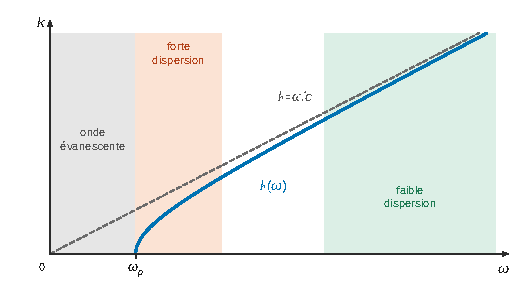
\includegraphics{figures/q05-courbe-dispersion.pdf}
\caption*{Figure 1 --- courbe de dispersion du plasma : coupure en ω\_p, asymptote
k = ω/c, zones de forte et de faible dispersion}
\end{figure}

\emph{Critère.} Un milieu est non dispersif quand \(v_\varphi\) ne dépend pas de \(\omega\). Cela revient à dire que \(k(\omega)\) est une droite passant par l'origine, et alors \(v_g=v_\varphi\).

On mesure la dispersion par l'écart de la courbe à la droite \(k=\omega/c\), ou par la variation de \(v_g\) avec \(\omega\).

\begin{itemize}
\tightlist
\item
  \textbf{Zone de forte dispersion} : \(\omega\) voisin de \(\omega_p\) (quelques \(\omega_p\)). La courbe s'écarte fortement de la droite et \(v_g\) varie très vite.
\item
  \textbf{Zone de faible dispersion} : \(\omega\gg\omega_p\). La courbe se confond avec l'asymptote, et \(v_g\simeq v_\varphi\simeq c\).
\end{itemize}

\textbf{b.} Un signal porteur de données n'est pas monochromatique : c'est un paquet d'ondes de largeur spectrale \(\Delta\omega\) d'autant plus grande que le débit est élevé. Dans un milieu dispersif, les composantes spectrales se propagent à des vitesses de groupe différentes. Le paquet s'étale au cours de la propagation, les impulsions successives se chevauchent (interférence entre symboles) et le signal est déformé. \textbf{La dispersion limite le débit et la fiabilité de la transmission.}

\textbf{c.} La bande Ku (\(10{,}7\) à \(14{,}5\) GHz) vérifie \(f/f_p\sim10^3\) :

\begin{itemize}
\tightlist
\item
  \(f\gg f_p\) : l'onde traverse l'ionosphère sans être réfléchie (Q3.d) ;
\item
  l'écart relatif \(1-v_g/c\simeq\dfrac{f_p^2}{2f^2}\sim3\times10^{-7}\) : la dispersion est négligeable, le signal n'est pas déformé (Q5.a et b) ;
\item
  une porteuse de haute fréquence autorise une large bande passante, donc un débit élevé, et des antennes directives de taille raisonnable.
\end{itemize}

\textbf{La bande Ku garantit une liaison transparente et quasi non dispersive à travers l'ionosphère.} (Au-delà de quelques dizaines de GHz, l'absorption par la vapeur d'eau et la pluie de la basse atmosphère devient gênante, ce qui borne le choix vers le haut.)

\begin{methode}

Dans un milieu de relation \(k(\omega)\), la dispersion se lit sur l'écart à une droite passant par l'origine. Elle est toujours forte près d'une coupure, où \(v_g\to0\).

\end{methode}

\begin{jury}

Les trois items de Q5 sont réussis par moins de 36 \% des candidats (figure 2a, p.~4). Le rapport 2026 (p.~5) l'explique de façon générale : « Les questions nécessitant une interprétation ou une explication physique des phénomènes présentent des taux de réussite relativement faibles. » En Q5.a, le critère de dispersion doit être énoncé, et pas seulement la courbe tracée. En Q5.c, chaque argument en faveur de la bande Ku doit être justifié.

\end{jury}

\hypertarget{partie-physique-2-points-de-lagrange-et-stabilituxe9}{%
\section{Partie Physique, 2 --- Points de Lagrange et stabilité}\label{partie-physique-2-points-de-lagrange-et-stabilituxe9}}

On établit les équations du mouvement d'un satellite dans le référentiel où le Soleil et la Terre sont fixes, puis on cherche les équilibres (points de Lagrange) et leur stabilité. Outils : référentiels non galiléens, énergie, gradient, linéarisation et valeurs propres.

\textbf{2.1 Étude préliminaire}

\hypertarget{question-6}{%
\subsection{Question 6}\label{question-6}}

\begin{indication}{1}

Appliquer le principe fondamental à la Terre dans le référentiel sidéral, où elle décrit un cercle centré sur le centre de masse \(O\).

\end{indication}

\begin{indication}{2}

Attention : le rayon de l'orbite de la Terre n'est pas \(R\). Exprimer \(OT\) en fonction de \(R\) et des masses par la définition du barycentre.

\end{indication}

\hypertarget{solution-5}{%
\subsubsection{Solution}\label{solution-5}}

\textbf{a.} Le système isolé \{S, T\} a son centre de masse \(O\) fixe dans le référentiel sidéral, qui est galiléen. La Terre décrit un cercle de rayon \(OT=R_T=\dfrac{M_S}{M}R\) à la vitesse angulaire \(\Omega\). Le principe fondamental appliqué à la Terre, projeté sur la direction radiale, donne

\equationajustee{M_T\,\Omega^2\,\frac{M_S}{M}R=\frac{GM_SM_T}{R^2},}

d'où, avec \(M=M_S+M_T\),

\equationajustee{\boxed{\Omega=\sqrt{\frac{GM}{R^3}}}}

C'est la troisième loi de Kepler pour le problème à deux corps.

\textbf{b.} \(T=\dfrac{2\pi}{\Omega}=2\pi\sqrt{\dfrac{R^3}{GM}}\) est la période de révolution commune de S et T autour de leur centre de masse, soit la période de révolution de la Terre autour du Soleil (avec \(M\simeq M_S\) et \(R=1\) UA) :

\equationajustee{\boxed{T\approx1\ \text{an}\approx3\times10^7\ \mathrm s}}

\begin{piege}

Écrire \(M_T\Omega^2R=GM_SM_T/R^2\) donne \(\Omega^2=GM_S/R^3\), ce qui est faux. Le rayon de l'orbite de T autour de \(O\) est en effet \(\frac{M_S}{M}R\), et non \(R\). Le résultat exact fait intervenir la masse totale.

\end{piege}

\hypertarget{question-7}{%
\subsection{Question 7}\label{question-7}}

\begin{indication}{1}

Écrire le principe fondamental dans \(\mathcal R_\Omega\) en ajoutant les forces d'inertie d'entraînement et de Coriolis ; la rotation est uniforme.

\end{indication}

\begin{indication}{2}

Exprimer chaque force qui n'est pas de Coriolis comme un gradient : potentiel newtonien en \(1/r\) pour chaque astre, potentiel centrifuge en \(r^2\).

\end{indication}

\begin{indication}{3}

Projeter sur \(\vec e_x\) et \(\vec e_y\) et identifier les termes de Coriolis avec ceux de (2) : leur signe doit correspondre.

\end{indication}

\hypertarget{solution-6}{%
\subsubsection{Solution}\label{solution-6}}

\textbf{a.} Le référentiel \(\mathcal R_\Omega\) tourne à la vitesse angulaire constante \(\vec\Omega=\Omega\vec e_z\). Son axe de rotation \((O,\vec e_\zeta)\) est fixe dans le référentiel galiléen \(\mathcal R_s\). Il n'y a donc pas de terme en \(\dot{\vec\Omega}\), et les forces d'inertie sont :

\begin{itemize}
\tightlist
\item
  la force d'inertie d'entraînement (centrifuge), \(-m\vec\Omega\wedge(\vec\Omega\wedge\overrightarrow{OP})=m\Omega^2\vec r\) pour \(\vec r\) dans le plan \((Oxy)\) ;
\item
  la force de Coriolis, \(-2m\vec\Omega\wedge\vec v\).
\end{itemize}

Le principe fondamental dans \(\mathcal R_\Omega\) s'écrit

\equationajustee{\ddot{\vec r}=-\frac{GM_S}{r_S^3}\vec r_S-\frac{GM_T}{r_T^3}\vec r_T+\Omega^2\vec r-2\Omega\vec e_z\wedge\dot{\vec r}.}

Le terme de Coriolis se projette en

\equationajustee{-2\Omega\vec e_z\wedge(\dot x\vec e_x+\dot y\vec e_y)=2\Omega\dot y\,\vec e_x-2\Omega\dot x\,\vec e_y .}

Les autres termes sont des gradients :

\equationajustee{\begin{aligned}
-\frac{GM_S}{r_S^3}\vec r_S&=\overrightarrow{\mathrm{grad}}\Big(\frac{GM_S}{r_S}\Big)\quad\text{(de \text{même} pour T)},\\
\Omega^2\vec r&=\overrightarrow{\mathrm{grad}}\Big(\frac12\Omega^2r^2\Big).
\end{aligned}}

La projection sur \(\vec e_x\) et \(\vec e_y\) donne

\equationajustee{\begin{aligned}
\ddot x-2\Omega\dot y&=\frac{\partial U}{\partial x},\\
\ddot y+2\Omega\dot x&=\frac{\partial U}{\partial y},
\end{aligned}}

avec la fonction \(U\) explicitée en b. Ce sont bien les équations (2).

\textbf{b.}

\equationajustee{\boxed{U(P)=\frac{GM_S}{r_S}+\frac{GM_T}{r_T}+\frac12\,\Omega^2r^2}}

\emph{Interprétation.} \(-mU\) est l'énergie potentielle dont dérivent les forces de gravitation du Soleil et de la Terre et la force d'inertie d'entraînement (énergie potentielle centrifuge \(-\tfrac12m\Omega^2r^2\)). La force de Coriolis ne dérive pas d'un potentiel mais ne travaille pas : \(U\) est l'opposé d'une énergie potentielle effective par unité de masse dans le référentiel tournant, d'où le nom de pseudo-potentiel.

\begin{methode}

Dans un référentiel en rotation uniforme autour d'un axe fixe, la force d'inertie d'entraînement dérive de l'énergie potentielle \(-\frac12m\Omega^2r_\perp^2\) (\(r_\perp\) distance à l'axe). La force de Coriolis ne dérive d'aucun potentiel mais ne travaille pas.

\end{methode}

\begin{piege}

Signes de Coriolis : avec \(\vec\Omega=\Omega\vec e_z\), le terme \(-2\vec\Omega\wedge\vec v\) a pour composante \(+2\Omega\dot y\) sur l'axe des abscisses. Sa composante sur l'axe des ordonnées vaut \(-2\Omega\dot x\). On vérifie par comparaison avec (2), qui est donnée.

\end{piege}

\begin{jury}

Selon le rapport 2026 (p.~6), la partie I.2 est « clairement » celle qui a posé le plus de difficultés. Les difficultés qu'il énumère commencent ici : « prise en compte des forces d'inertie dans un référentiel tournant, interprétation du pseudo-potentiel et de la constante de Jacobi ». Q7.a est réussie par environ 38 \% des candidats, Q7.b (expression et interprétation de \(U\)) par 8 \% seulement (figure 2b, p.~4).

\end{jury}

\hypertarget{question-8}{%
\subsection{Question 8}\label{question-8}}

\begin{indication}{1}

Pour faire apparaître une intégrale première, faire le produit scalaire des équations du mouvement avec la vitesse.

\end{indication}

\begin{indication}{2}

Que devient le travail de la force de Coriolis ? Pour (b), utiliser le fait qu'un carré de vitesse est positif.

\end{indication}

\hypertarget{solution-7}{%
\subsubsection{Solution}\label{solution-7}}

\textbf{a.} On multiplie la première équation (2) par \(\dot x\), la seconde par \(\dot y\), et on somme. Les termes de Coriolis se compensent (\(-2\Omega\dot x\dot y+2\Omega\dot y\dot x=0\)) :

\equationajustee{\dot x\ddot x+\dot y\ddot y=\frac{\partial U}{\partial x}\dot x+\frac{\partial U}{\partial y}\dot y,}

soit, puisque \(U\) ne dépend pas explicitement du temps dans \(\mathcal R_\Omega\),

\equationajustee{\frac{\mathrm d}{\mathrm dt}\Big(\frac{v^2}{2}\Big)=\frac{\mathrm dU}{\mathrm dt}.}

Donc

\equationajustee{\boxed{C_J=2U-v^2=\text{constante du mouvement}}}

\emph{Interprétation.} \(E=\tfrac12mv^2-mU=-\tfrac m2C_J\) est l'énergie mécanique de P dans le référentiel tournant, en incluant l'énergie potentielle centrifuge. Elle se conserve parce que la force de Coriolis, perpendiculaire à la vitesse, ne travaille pas. La constante de Jacobi est, au facteur \(-m/2\) près, cette énergie mécanique.

\textbf{b.} Comme \(v^2=2U-C_J\ge0\), le point P ne peut occuper que les points où \(U(P)\ge C_J/2\). \textbf{Les zones d'exclusion sont les régions où \(U<C_J/2\).}

Elles sont délimitées par les courbes de vitesse nulle \(U=C_J/2\), qui sont des lignes de niveau de \(U\) comme celles de la figure 2. La valeur de \(C_J\) est fixée par les conditions initiales (position et vitesse dans \(\mathcal R_\Omega\)). Par exemple, si \(C_J/2>U(\mathrm L_1)\), un satellite lancé près de la Terre reste confiné dans la région entourant la Terre, sans pouvoir passer vers le Soleil.

\begin{methode}

Multiplier une équation du mouvement par la vitesse, c'est appliquer le théorème de l'énergie cinétique. Une force perpendiculaire à la vitesse (Coriolis, force magnétique) disparaît toujours de ce bilan.

\end{methode}

\begin{jury}

Le rapport 2026 découpe Q8.a en deux items (« Q8-a1 », « Q8-a2 »), vraisemblablement l'existence de \(C_J\) et son interprétation. Ils sont réussis par environ 14 \% et 5 \% des candidats, et Q8.b par 10 \% (figure 2b, p.~4). L'interprétation énergétique, notée à part, ne doit donc pas être sacrifiée au calcul.

\end{jury}

\textbf{2.2 Détermination des positions des points de Lagrange}

\hypertarget{question-9}{%
\subsection{Question 9}\label{question-9}}

\begin{indication}{1}

Construire les unités dérivées (vitesse angulaire, constante de gravitation) à partir de \(u_M\), \(u_L\) et \(u_t\), par analyse dimensionnelle.

\end{indication}

\begin{indication}{2}

Utiliser la relation obtenue en Q6.a pour simplifier l'unité de \(G\).

\end{indication}

\hypertarget{solution-8}{%
\subsubsection{Solution}\label{solution-8}}

\textbf{a.} L'unité de vitesse angulaire est \(u_\Omega=1/u_t\). Or \(1/u_t=2\pi/T=\Omega\), donc \(u_\Omega=\Omega\).

D'après la dimension de \(G\) (\(\mathrm{m^3\,kg^{-1}\,s^{-2}}\)), son unité est

\equationajustee{\begin{aligned}
u_G&=\frac{u_L^3}{u_Mu_t^2}\\
&=\frac{R^3\Omega^2}{M}\\
&=G\quad\text{d'\text{après} Q6.a.}
\end{aligned}}

Donc

\equationajustee{\begin{aligned}
\omega&=\frac{\Omega}{u_\Omega}=\boxed{1},\\
\Gamma&=\frac{G}{u_G}\\
&=\frac{GM}{R^3\Omega^2}\\
&=\boxed{1}.
\end{aligned}}

\textbf{b.} Par définition de \(u_t\),

\equationajustee{\begin{aligned}
\tau&=\frac{t}{u_t}\\
&=\frac{2\pi t}{T}\\
&=\Omega t .
\end{aligned}}

Or l'axe \(\vec e_x\) du référentiel synodique est porté par \(\overrightarrow{ST}\). Il tourne à la vitesse angulaire \(\Omega\) et coïncide avec \(\vec e_\xi\) à \(t=0\). Donc \(\theta=(\vec e_\xi,\vec e_x)=\Omega t\) et

\equationajustee{\boxed{\tau=\theta}}

Le temps adimensionné mesure l'angle dont a tourné le système Soleil--Terre ; un tour complet correspond à \(\tau=2\pi\), soit un an.

\hypertarget{question-10}{%
\subsection{Question 10}\label{question-10}}

\begin{indication}{1}

Placer S et T sur l'axe \(\tilde x\) (barycentre à l'origine). Exprimer ensuite \(\rho_S\) et \(\rho_T\) en fonction de \((\tilde x,\tilde y)\).

\end{indication}

\begin{indication}{2}

Dériver par composition : \(\partial\tilde U/\partial\tilde x=\frac{\mathrm d\tilde U}{\mathrm d\rho_S}\frac{\partial\rho_S}{\partial\tilde x}+\dots\), et noter qu'une même fonction de \(\rho\) apparaît pour les deux astres.

\end{indication}

\begin{indication}{3}

Avec \(\tilde y\neq0\), combiner les deux conditions d'équilibre pour séparer la contribution du Soleil de celle de la Terre.

\end{indication}

\hypertarget{solution-9}{%
\subsubsection{Solution}\label{solution-9}}

Le centre de masse étant à l'origine, S est en \((-\mu_T,0)\) et T en \((\mu_S,0)\), avec \(\mu_S+\mu_T=1\) :

\equationajustee{\begin{aligned}
\rho_S^2&=(\tilde x+\mu_T)^2+\tilde y^2,\\
\rho_T^2&=(\tilde x-\mu_S)^2+\tilde y^2 .
\end{aligned}}

Notons \(f(\rho)=\rho-\dfrac1{\rho^2}\), de sorte que \(\dfrac{\mathrm d}{\mathrm d\rho}\Big(\dfrac1\rho+\dfrac{\rho^2}2\Big)=f(\rho)\). On a \(\dfrac{\partial\rho_S}{\partial\tilde x}=\dfrac{\tilde x+\mu_T}{\rho_S}\) et \(\dfrac{\partial\rho_S}{\partial\tilde y}=\dfrac{\tilde y}{\rho_S}\), et de même pour T. Par dérivation composée :

\equationajustee{\begin{aligned}
\frac{\partial\tilde U}{\partial\tilde x}&=\mu_S\frac{f(\rho_S)}{\rho_S}(\tilde x+\mu_T)+\mu_T\frac{f(\rho_T)}{\rho_T}(\tilde x-\mu_S),\\
\frac{\partial\tilde U}{\partial\tilde y}&=\tilde y\Big[\mu_S\frac{f(\rho_S)}{\rho_S}+\mu_T\frac{f(\rho_T)}{\rho_T}\Big].
\end{aligned}}

Pour un équilibre hors de l'axe (\(\tilde y\neq0\)), la seconde condition donne

\equationajustee{\mu_S\frac{f(\rho_S)}{\rho_S}+\mu_T\frac{f(\rho_T)}{\rho_T}=0 .}

En retranchant \(\tilde x\) fois cette relation à la première, on obtient

\equationajustee{\mu_S\mu_T\Big[\frac{f(\rho_S)}{\rho_S}-\frac{f(\rho_T)}{\rho_T}\Big]=0 .}

Les deux termes sont donc égaux, et chacun est nul puisque leur combinaison à coefficients positifs l'est. Ainsi \(f(\rho_S)=f(\rho_T)=0\) :

\equationajustee{\boxed{\rho_S=\rho_T=1}}

\(\mathrm L_4\) et \(\mathrm L_5\) sont à la distance \(R\) du Soleil et de la Terre : ils forment avec S et T deux \textbf{triangles équilatéraux}. L'égalité \((\tilde x+\mu_T)^2=(\tilde x-\mu_S)^2\) donne \(\tilde x=\dfrac{\mu_S-\mu_T}{2}\), puis \(\tilde y^2=1-\dfrac14\) :

\equationajustee{\boxed{\begin{aligned}
\mathrm L_4\ :\ (\tilde x,\tilde y)&=\Big(\frac12-\mu_T,\ \frac{\sqrt3}2\Big)\\
\mathrm L_5\ :\ (\tilde x,\tilde y)&=\Big(\frac12-\mu_T,\ -\frac{\sqrt3}2\Big)\\
\mathrm L_4,\ \mathrm L_5\ :\ (\rho_S,\rho_T)&=(1,1)
\end{aligned}}}

(\(\mathrm L_4\) est au-dessus de l'axe sur la figure 2, en avance sur la Terre dans le sens de rotation.) On vérifie \(\tilde U(\mathrm L_4)=\tfrac32-\tfrac12\mu_S\mu_T\), soit \(1{,}42\) pour \(\mu_T=0{,}2\), valeur de la légende.

\begin{piege}

L'énoncé insiste : les distances \(\rho_S\) et \(\rho_T\) dépendent de la position \((\tilde x,\tilde y)\). Annuler « \(\partial\tilde U/\partial\rho_S\) » sans dérivée composée donne le bon résultat par chance, mais sans démonstration. Il faut aussi montrer que les deux termes s'annulent séparément.

\end{piege}

\begin{jury}

Q10 n'est réussie que par environ 5 \% des candidats, Q11 par 3 \% au plus (figure 2b, p.~4). Le rapport 2026 (p.~6) cite parmi les difficultés le « changement de variables et adimensionnement » et la « géométrie des points de Lagrange ». L'énoncé met lui-même en garde contre l'oubli de la dépendance de \(\rho_S\) et \(\rho_T\) en \((\tilde x,\tilde y)\).

\end{jury}

\hypertarget{question-11}{%
\subsection{Question 11}\label{question-11}}

\begin{indication}{1}

Entre S et T sur l'axe, les distances aux deux astres s'additionnent : que vaut \(\rho_S+\rho_T\) ?

\end{indication}

\begin{indication}{2}

Écrire \(\partial\tilde U/\partial\tilde x=0\) avec les bons signes de \(\partial\rho/\partial\tilde x\). Factoriser ensuite \((1-\rho_T)^3-1\) et \(1-\rho_T^3\).

\end{indication}

\hypertarget{solution-10}{%
\subsubsection{Solution}\label{solution-10}}

\(\mathrm L_1\) est sur l'axe (\(\tilde y_1=0\)) entre S et T, donc \(-\mu_T<\tilde x_1<\mu_S\) et

\equationajustee{\begin{aligned}
\rho_S&=\tilde x_1+\mu_T,\\
\rho_T&=\mu_S-\tilde x_1,
\end{aligned}}

d'où \(\rho_S+\rho_T=1\).

Sur ce segment, \(\partial\tilde U/\partial\tilde y=0\) par symétrie. De plus \(\dfrac{\partial\rho_S}{\partial\tilde x}=1\) et \(\dfrac{\partial\rho_T}{\partial\tilde x}=-1\). L'équilibre \(\partial\tilde U/\partial\tilde x=0\) s'écrit donc

\equationajustee{\mu_S f(\rho_S)=\mu_T f(\rho_T),}

avec \(\rho_S=1-\rho_T\). On factorise :

\equationajustee{\begin{aligned}
f(1-\rho_T)&=\frac{(1-\rho_T)^3-1}{(1-\rho_T)^2}\\
&=-\frac{\rho_T\,(3-3\rho_T+\rho_T^2)}{(1-\rho_T)^2},\\
f(\rho_T)&=\frac{\rho_T^3-1}{\rho_T^2}\\
&=-\frac{1-\rho_T^3}{\rho_T^2}.
\end{aligned}}

En reportant :

\equationajustee{\mu_S\,\frac{3\rho_T\big(1-\rho_T+\rho_T^2/3\big)}{(1-\rho_T)^2}=\mu_T\,\frac{1-\rho_T^3}{\rho_T^2},}

soit

\equationajustee{\boxed{\frac{\mu_T}{3\mu_S}=\rho_T^3\,\frac{1-\rho_T+\dfrac{\rho_T^2}{3}}{(1-\rho_T)^2(1-\rho_T^3)}}\qquad(5)}

\begin{methode}

Sur l'axe, \(\partial\rho/\partial\tilde x=\pm1\) selon le côté de l'astre où l'on se trouve. Pour \(\mathrm L_2\) (au-delà de T) ou \(\mathrm L_3\) (au-delà de S), les signes changent et l'on obtient d'autres équations de la même famille.

\end{methode}

\hypertarget{question-12}{%
\subsection{Question 12}\label{question-12}}

\begin{indication}{1}

Calculer \(\alpha\) ; il est très petit, donc \(\rho_T\) aussi. Quels facteurs de (5) valent alors à peu près 1 ?

\end{indication}

\hypertarget{solution-11}{%
\subsubsection{Solution}\label{solution-11}}

\textbf{a.} Application numérique :

\equationajustee{\begin{aligned}
\alpha&=\frac{\mu_T}{3\mu_S}\\
&=\frac{M_T}{3M_S}\\
&=\frac{6{,}0\times10^{24}}{3\times2{,}0\times10^{30}}\\
&=\boxed{1{,}0\times10^{-6}}
\end{aligned}}

Comme \(\alpha\ll1\), on a \(\rho_T\ll1\), et le membre de droite de (5) vaut \(\rho_T^3\big(1+O(\rho_T)\big)\). Au plus bas ordre, \(\rho_T^3\simeq\alpha\) :

\equationajustee{\boxed{\rho_T\simeq\alpha^{1/3}=1\times10^{-2}}}

(La correction suivante est d'ordre relatif \(\rho_T/3\approx0{,}3\,\%\) ; la racine exacte de (5) vaut \(\rho_T\approx0{,}00997\).)

\textbf{b.}

\equationajustee{\boxed{r_T=\rho_T\,R\simeq10^{-2}\times1{,}5\times10^{11}=1{,}5\times10^{9}\ \mathrm m}}

soit environ \(1{,}5\) million de kilomètres, quatre fois la distance Terre--Lune : c'est la position de SoHO, WIND et SMILE.

\begin{methode}

Le rayon de la sphère de Hill, \(r\simeq R\,(M_T/3M_S)^{1/3}\), est un ordre de grandeur à connaître : c'est la taille de la zone d'influence gravitationnelle d'une planète.

\end{methode}

\begin{jury}

Q12 se traite sans avoir démontré (5), puisque l'équation est donnée. Elle reste pourtant peu réussie : environ 15 \% pour Q12.a et 9 \% pour Q12.b (figure 2b, p.~4). C'est typiquement une question à prendre même si Q11 a résisté.

\end{jury}

\textbf{2.3 Étude de la stabilité des points de Lagrange}

\hypertarget{question-13}{%
\subsection{Question 13}\label{question-13}}

\begin{indication}{1}

Regarder la figure 2 : que se passe-t-il pour les lignes de niveau au voisinage de \(\mathrm L_1\), \(\mathrm L_2\) et \(\mathrm L_3\) ? Quel type de point critique cela révèle-t-il ?

\end{indication}

\begin{indication}{2}

Relier la forme de \(U\) à celle de \(E_p=-mU\) et raisonner sur un petit déplacement dans la direction défavorable.

\end{indication}

\hypertarget{solution-12}{%
\subsubsection{Solution}\label{solution-12}}

Sur la figure 2, les lignes de niveau ①, ② et ③ se \textbf{croisent} respectivement en \(\mathrm L_1\), \(\mathrm L_2\) et \(\mathrm L_3\). Un point où une ligne de niveau se recoupe est un \textbf{point-col}.

Le long de l'axe S--T, \(\tilde U\) est minimale en ce point : elle tend vers \(+\infty\) de part et d'autre (près d'un astre, ou loin des deux par le terme centrifuge). Dans la direction perpendiculaire, elle est maximale : elle décroît vers \(\mathrm L_4\) et \(\mathrm L_5\), où elle est minimale.

Comme \(E_p=-mU\), l'énergie potentielle présente elle aussi un col : il existe une direction le long de laquelle \(E_p\) est maximale. Un petit écart dans cette direction fait apparaître une force qui éloigne P de l'équilibre.

La force de Coriolis ne peut pas rattraper cela. Avec les notations de Q15, un col donne \(U_{xx}U_{yy}-U_{xy}^2<0\). Le produit des racines en \(\lambda^2\) est alors négatif, d'où une racine \(\lambda\) réelle positive, c'est-à-dire un écart qui croît exponentiellement. \textbf{\(\mathrm L_1\), \(\mathrm L_2\) et \(\mathrm L_3\) sont instables.}

\begin{piege}

Ne pas conclure « \(U\) est maximale en \(\mathrm L_1\) » ni « minimale » : c'est un col.~Le croisement des lignes de niveau sur la figure 2 en est la signature graphique.

\end{piege}

\begin{jury}

Le rapport 2026 (p.~6) range la fin de la partie parmi les difficultés cumulées : « développement limité puis analyse de stabilité à partir des valeurs propres ». De Q13 à Q17, aucun item ne dépasse 12 \% de réussite (figure 2b, p.~4), et Q17 n'est abordée que par environ 2 \% des candidats (figure 1b, p.~2). Le rapport précise que ce faible taux de réponse « ne peut pas être attribué uniquement à un manque de temps ».

\end{jury}

\hypertarget{question-14}{%
\subsection{Question 14}\label{question-14}}

\begin{indication}{1}

La force de Coriolis est perpendiculaire à la vitesse : que fait-elle à la trajectoire, et que fait-elle à l'énergie ?

\end{indication}

\begin{indication}{2}

Penser aux mouvements atmosphériques autour d'une dépression dans le référentiel terrestre.

\end{indication}

\hypertarget{solution-13}{%
\subsubsection{Solution}\label{solution-13}}

En \(\mathrm L_4\), \(E_p\) est maximale : sans autre force, un satellite écarté de \(\mathrm L_4\) « dévalerait » la colline de potentiel.

Mais dès qu'il prend une vitesse \(\vec v\) dans \(\mathcal R_\Omega\), la force de Coriolis \(-2m\vec\Omega\wedge\vec v\) intervient. Perpendiculaire à la vitesse et d'intensité proportionnelle à \(v\), elle courbe la trajectoire sans modifier l'énergie. Pour \(\vec\Omega\) selon \(+\vec e_z\), elle dévie le mouvement vers la droite.

La chute vers l'extérieur est ainsi convertie en un mouvement de rotation autour de \(\mathrm L_4\), à la manière d'un cyclone qui tourne autour d'une dépression au lieu de la combler. Si la force de Coriolis est assez grande devant la force « répulsive » due au potentiel, la trajectoire reste confinée au voisinage de \(\mathrm L_4\) : c'est une \textbf{stabilité dynamique}, assurée par le mouvement et non par un minimum d'énergie potentielle.

\begin{piege}

La force de Coriolis ne peut pas créer un puits de potentiel, puisqu'elle ne travaille pas. Elle stabilise en courbant la trajectoire, et seulement si elle est assez intense : c'est l'objet de la condition sur \(\mu_T\) en Q16.

\end{piege}

\hypertarget{question-15}{%
\subsection{Question 15}\label{question-15}}

\begin{indication}{1}

Écrire les dérivées premières de \(\tilde U\) à l'ordre 1 en \((X,Y)\) autour de l'équilibre : que valent-elles au point d'équilibre lui-même ?

\end{indication}

\begin{indication}{2}

Les deux premières lignes de \(\mathbf A\) sont triviales (définition des vitesses) ; les deux dernières recopient (7).

\end{indication}

\hypertarget{solution-14}{%
\subsubsection{Solution}\label{solution-14}}

Au point d'équilibre \((x_0,y_0)\), les dérivées premières de \(\tilde U\) sont nulles. Le développement de \(\tilde U\) à l'ordre 2 donne, à l'ordre 1 en \(X\) et \(Y\) :

\equationajustee{\begin{aligned}
\frac{\partial\tilde U}{\partial X}&=U_{xx}X+U_{xy}Y,\\
\frac{\partial\tilde U}{\partial Y}&=U_{xy}X+U_{yy}Y .
\end{aligned}}

Les équations (7) deviennent

\equationajustee{\begin{aligned}
X''&=U_{xx}X+U_{xy}Y+2Y',\\
Y''&=U_{xy}X+U_{yy}Y-2X',
\end{aligned}}

soit

\equationajustee{\begin{pmatrix}X'\\Y'\\X''\\Y''\end{pmatrix}=\mathbf A\begin{pmatrix}X\\Y\\X'\\Y'\end{pmatrix},}

avec

\equationajustee{\boxed{\mathbf A=\begin{pmatrix}0&0&1&0\\0&0&0&1\\U_{xx}&U_{xy}&0&2\\U_{xy}&U_{yy}&-2&0\end{pmatrix}}}

Son polynôme caractéristique est

\equationajustee{\chi_{\mathbf A}(\lambda)=\lambda^4+(4-U_{xx}-U_{yy})\lambda^2+U_{xx}U_{yy}-U_{xy}^2 .}

En \(\mathrm L_4\), les dérivées secondes valent

\equationajustee{\begin{aligned}
U_{xx}&=\tfrac34,\\
U_{yy}&=\tfrac94,\\
U_{xy}&=\tfrac{3\sqrt3}{4}(1-2\mu_T),
\end{aligned}}

ce qui redonne bien l'équation (10).

\begin{methode}

Linéariser un système du second ordre autour d'un équilibre puis l'écrire sous forme d'état \(\mathbf Y'=\mathbf A\mathbf Y\) ramène l'étude de stabilité au spectre de \(\mathbf A\).

\end{methode}

\hypertarget{question-16}{%
\subsection{Question 16}\label{question-16}}

\begin{indication}{1}

Poser \(\Lambda=\lambda^2\). À quelle condition sur les \(\lambda_k\) les solutions (9) restent-elles bornées ?

\end{indication}

\begin{indication}{2}

Utiliser la somme et le produit des racines \(\Lambda\) pour conclure sur leur signe quand elles sont réelles, et ne pas oublier le cas d'une racine double.

\end{indication}

\hypertarget{solution-15}{%
\subsubsection{Solution}\label{solution-15}}

\textbf{a.} On pose \(\Lambda=\lambda^2\) :

\equationajustee{\Lambda^2+\Lambda+\frac{27}4\mu_T(1-\mu_T)=0 .}

Le mouvement (9) reste borné si et seulement si les quatre \(\lambda_k\) sont imaginaires purs et distincts. En effet, une partie réelle positive donne une divergence exponentielle, et une racine double donne des termes séculaires en \(\tau\,\mathrm e^{\lambda\tau}\). Il faut donc deux racines \(\Lambda\) réelles, strictement négatives et distinctes.

\begin{itemize}
\tightlist
\item
  Elles sont réelles et distinctes si le discriminant est strictement positif : \(1-27\mu_T(1-\mu_T)>0\).
\item
  Leur somme vaut \(-1<0\) et leur produit \(\frac{27}4\mu_T(1-\mu_T)>0\) : si elles sont réelles, elles sont toutes deux négatives.
\item
  Si le discriminant est négatif, les \(\Lambda\) sont complexes conjugués non réels, et parmi les \(\lambda=\pm\sqrt\Lambda\) l'un a une partie réelle positive : instabilité.
\end{itemize}

\equationajustee{\boxed{27\,\mu_T(1-\mu_T)<1\iff\mu_T<\frac{1-\sqrt{23/27}}{2}\approx0{,}0385}}

(\(\mu_T\) désigne la plus petite des deux masses réduites ; c'est le critère de Routh.)

\textbf{b.} Application numérique :

\equationajustee{\begin{aligned}
\mu_T&=\frac{M_T}{M_S+M_T}\\
&\simeq\frac{M_T}{M_S}\\
&=\frac{6{,}0\times10^{24}}{2{,}0\times10^{30}}\\
&=3{,}0\times10^{-6}\ll0{,}04 .
\end{aligned}}

\textbf{La condition est très largement satisfaite : \(\mathrm L_4\) et \(\mathrm L_5\) sont dynamiquement stables pour le système Soleil--Terre}, ce qui est cohérent avec les troyens terrestres observés.

\begin{methode}

Pour un système conservatif linéarisé, la stabilité impose des valeurs propres imaginaires pures. Avec une équation bicarrée, on raisonne sur \(\Lambda=\lambda^2\) : il faut deux racines réelles strictement négatives et distinctes.

\end{methode}

\hypertarget{question-17}{%
\subsection{Question 17}\label{question-17}}

\begin{indication}{1}

Avec \(\mu_T\ll1\), résoudre l'équation en \(\Lambda\) par un développement limité : une racine proche de \(-1\), l'autre très petite.

\end{indication}

\begin{indication}{2}

Convertir les pulsations adimensionnées en périodes réelles : à quelle durée correspond une unité de \(\tau\) ?

\end{indication}

\hypertarget{solution-16}{%
\subsubsection{Solution}\label{solution-16}}

On pose

\equationajustee{\begin{aligned}
\varepsilon&=\frac{27}{4}\mu_T(1-\mu_T)\\
&\simeq\frac{27}{4}\times3{,}0\times10^{-6}\\
&\approx2{,}0\times10^{-5}\ll1 .
\end{aligned}}

Les racines de \(\Lambda^2+\Lambda+\varepsilon=0\) sont alors

\equationajustee{\begin{aligned}
\Lambda_1&\simeq-1+\varepsilon\simeq-1,\\
\Lambda_2&\simeq-\varepsilon\approx-2{,}0\times10^{-5}.
\end{aligned}}

Les solutions sont donc des combinaisons de deux oscillations de pulsations adimensionnées distinctes :

\equationajustee{\begin{aligned}
\omega_1&=\sqrt{-\Lambda_1}\simeq1,\\
\omega_2&=\sqrt{-\Lambda_2}\\
&=\sqrt{\tfrac{27}4\mu_T}\\
&\approx\sqrt{20\times10^{-6}}\\
&\approx4{,}5\times10^{-3}.
\end{aligned}}

Le mouvement est la superposition de deux oscillations de périodes différentes. Les exponentielles de (9) s'entendent en temps adimensionné \(\tau=\Omega t\). Une pulsation adimensionnée \(\omega_k\) correspond donc à la pulsation réelle \(\omega_k\Omega\).

La période correspondante est \(T_k=\dfrac{2\pi}{\omega_k\Omega}=\dfrac{T}{\omega_k}\), avec \(T=1\) an :

\equationajustee{\boxed{\begin{aligned}
T_1&=\frac{T}{\omega_1}\approx1\ \text{an}\\
T_2&=\frac{T}{\omega_2}\approx\frac{1\ \text{an}}{4{,}5\times10^{-3}}\approx2{,}2\times10^{2}\ \text{ans}
\end{aligned}}}

On a bien \(T_2>T_1\) : le satellite décrit une petite boucle annuelle (épicycle) dont le centre dérive lentement autour de \(\mathrm L_4\) avec une période d'environ deux siècles (libration).

\begin{piege}

Les pulsations obtenues sont sans dimension, puisque le temps de (9) est \(\tau\). Oublier le facteur \(u_t=T/2\pi\) conduit à des « périodes » de \(2\pi\) et \(1400\) sans unité.

\end{piege}

\hypertarget{partie-si-2-duxe9ploiement-des-panneaux-solaires}{%
\section{Partie SI, 2 --- Déploiement des panneaux solaires}\label{partie-si-2-duxe9ploiement-des-panneaux-solaires}}

On modélise le mécanisme de déploiement d'un panneau, on établit ses équations du mouvement par le principe fondamental de la dynamique, puis on confronte une simulation au cahier des charges. Outils : graphe de liaisons, cinématique du solide, opérateur d'inertie, torseurs cinétique et dynamique.

\textbf{2.1 Analyse du mécanisme}

\hypertarget{question-18}{%
\subsection{Question 18}\label{question-18}}

\begin{indication}{1}

Lister les solides, puis traduire chaque charnière en liaison normalisée d'après ses mobilités (« les 3 rotations de l'espace »).

\end{indication}

\begin{indication}{2}

Entre deux panneaux, combien de charnières y a-t-il ?

\end{indication}

\hypertarget{solution-17}{%
\subsubsection{Solution}\label{solution-17}}

Solides : satellite 0, arbre 1, bras 2, panneaux 3, 4 et 5. Liaisons (« les 3 rotations de l'espace » d'une charnière donnent une liaison \textbf{sphérique}) :

\begin{longtable}[]{@{}
  >{\raggedright\arraybackslash}p{(\columnwidth - 2\tabcolsep) * \real{0.2125}}
  >{\raggedright\arraybackslash}p{(\columnwidth - 2\tabcolsep) * \real{0.7575}}@{}}
\toprule\noalign{}
\begin{minipage}[b]{\linewidth}\raggedright
Solides
\end{minipage} & \begin{minipage}[b]{\linewidth}\raggedright
Liaison
\end{minipage} \\
\midrule\noalign{}
\endhead
\bottomrule\noalign{}
\endlastfoot
0--1 & pivot d'axe \((O_1,\vec x_1)\) \\
1--2 & pivot d'axe \((O_2,\vec z_2)\) (charnière principale) \\
2--3 & sphérique de centre \(J_3\) (charnière passive) et sphérique de centre \(I_3\) (charnière active) \\
3--4 & sphérique de centre \(J_4\) et sphérique de centre \(I_4\) \\
4--5 & sphérique de centre \(J_5\) et sphérique de centre \(I_5\) \\
\end{longtable}

\begin{figure}[H]
\centering
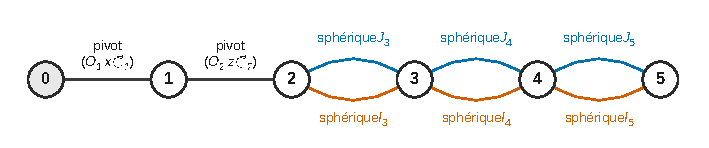
\includegraphics{figures/q18-graphe-liaisons.pdf}
\caption*{Figure 2 --- graphe de liaisons : deux pivots, puis deux sphériques J et
I en parallèle entre solides successifs}
\end{figure}

Entre deux panneaux successifs, il y a deux arcs en parallèle (deux sphériques). Le graphe est une chaîne ouverte dont chaque étage panneau--panneau forme une boucle fermée.

\begin{piege}

Ne pas remplacer d'emblée les deux charnières par une pivot dans le graphe : le graphe doit représenter les liaisons réelles. L'équivalence se discute ensuite.

\end{piege}

\begin{jury}

Pour II.1, le rapport 2026 (p.~6--7) situe les difficultés dans « la lecture du mécanisme tridimensionnel et l'identification correcte des liaisons et de leurs degrés de liberté ». Q18 est réussie par environ 62 \% des candidats (figure 2c, p.~5).

\end{jury}

\hypertarget{question-19}{%
\subsection{Question 19}\label{question-19}}

\begin{indication}{1}

Le dessiner en configuration déployée : tous les axes de charnière sont alors parallèles.

\end{indication}

\begin{indication}{2}

Utiliser les symboles normalisés et indiquer les axes et les centres. Quelle liaison équivalente forment deux liaisons sphériques entre les mêmes solides ?

\end{indication}

\hypertarget{solution-18}{%
\subsubsection{Solution}\label{solution-18}}

Schéma cinématique en configuration déployée, dessiné dans le plan des panneaux (\(\vec x_1\) horizontal, \(\vec z_2\) vertical) :

\begin{figure}[H]
\centering
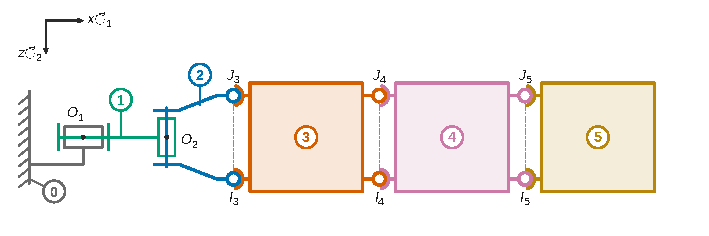
\includegraphics{figures/q19-schema-cinematique.pdf}
\caption*{Figure 3 --- schéma cinématique en configuration déployée, dans le plan
des panneaux}
\end{figure}

\begin{itemize}
\tightlist
\item
  La pivot d'axe \((O_1,\vec x_1)\) (palier lié au bâti 0, arbre 1 à deux épaulements) est dessinée le long de l'axe de l'arbre.
\item
  La pivot d'axe \((O_2,\vec z_2)\) relie l'arbre 1 au bras 2. Son axe \(\vec z_2\) est \textbf{dans le plan des panneaux}, parallèle aux arêtes de charnière.
\item
  Chaque charnière entre deux solides successifs est représentée par deux liaisons sphériques de centres \(J_i\) et \(I_i\), alignées sur l'arête commune, parallèle à \(\vec z_2\) pendant le déploiement.
\end{itemize}

Deux sphériques en parallèle de centres distincts sont équivalentes à une \textbf{pivot d'axe \((J_iI_i)\)}. C'est ce qui justifie la modélisation de la partie 2.2 (pivot d'axe \((O_3,\vec z_0)\) entre 2 et 3). Cette association est hyperstatique de degré 1 (6 inconnues statiques pour 5 mobilités bloquées) : la translation le long de \(J_iI_i\) est bloquée deux fois.

\begin{methode}

Deux liaisons en parallèle entre deux mêmes solides : on cherche la liaison équivalente par les mobilités communes (intersection des torseurs cinématiques). Deux sphériques de centres distincts donnent une pivot d'axe la droite des centres.

\end{methode}

\begin{piege}

Le schéma demandé est celui du mécanisme de la figure 4, avec l'arbre 1, le bras 2 et les trois panneaux. Il ne faut pas se contenter du modèle plan à deux pivots de la figure 5, qui n'est introduit qu'en 2.2.

\end{piege}

\begin{jury}

« Le passage du système réel représenté figure 4 à un modèle cinématique constitue ici la principale source d'erreur. Q19, consacrée au schéma cinématique, est d'ailleurs sensiblement moins abordée et moins réussie que Q18. » (rapport 2026, p.~7). Environ 31 \% de réussite, contre 62 \% pour Q18 (figure 2c, p.~5).

\end{jury}

\textbf{2.2 Dynamique du déploiement}

\hypertarget{question-20}{%
\subsection{Question 20}\label{question-20}}

\begin{indication}{1}

Le satellite est en orbite : son mouvement par rapport à un référentiel héliocentrique est-il une translation rectiligne uniforme ?

\end{indication}

\begin{indication}{2}

Pour l'approximation, penser à la chute libre (qu'est-ce qui compense la force d'inertie de translation ?), aux échelles de temps et au rapport des masses.

\end{indication}

\hypertarget{solution-19}{%
\subsubsection{Solution}\label{solution-19}}

\(\mathcal R_0\) est lié au satellite, qui est en orbite (au voisinage de \(\mathrm L_1\)) et peut tourner sur lui-même. Il est accéléré par rapport au référentiel héliocentrique : \textbf{il n'est pas galiléen}. On peut l'assimiler à un référentiel galiléen pour le déploiement car :

\begin{itemize}
\tightlist
\item
  \textbf{translation} : le satellite est en chute libre. La force d'inertie d'entraînement de translation \(-m\vec a(O_0)\) compense la gravitation, quasi uniforme à l'échelle du mécanisme (quelques mètres). Les termes de marée sont négligeables. Négliger la gravité, comme le fait l'énoncé, n'est cohérent qu'avec cet argument ;
\item
  \textbf{rotation} : la rotation de \(\mathcal R_0\) (orbitale, \(\Omega_{\text{orb}}\approx2\times10^{-7}\ \mathrm{rad\,s^{-1}}\), ou d'attitude, lente et contrôlée) est négligeable à l'échelle des 8 s du déploiement : les forces centrifuge et de Coriolis sont infimes devant les actions des ressorts ;
\item
  \textbf{recul du satellite} : la masse du satellite (de l'ordre de la tonne) est très grande devant celle du bras et des panneaux (quelques kilogrammes). Le mouvement du corps 0 induit par le déploiement est négligeable.
\end{itemize}

\begin{piege}

Dire que la force d'inertie de translation est négligeable est faux. Près de \(\mathrm L_1\), l'accélération du satellite est d'environ \(6\times10^{-3}\ \mathrm{m\,s^{-2}}\). Elle donne sur le panneau un moment d'environ \(0{,}03\ \mathrm{N\,m}\), non négligeable devant celui des ressorts (au plus \(0{,}16\ \mathrm{N\,m}\)). Elle est en réalité compensée par la gravitation (chute libre).

\end{piege}

\hypertarget{question-21}{%
\subsection{Question 21}\label{question-21}}

\begin{indication}{1}

Identifier les plans de symétrie du panneau pour justifier la forme diagonale.

\end{indication}

\begin{indication}{2}

Le moment d'inertie par rapport à un axe fait intervenir les deux dimensions perpendiculaires à cet axe.

\end{indication}

\hypertarget{solution-20}{%
\subsubsection{Solution}\label{solution-20}}

Le panneau 3 est un parallélépipède homogène de dimensions :

\begin{itemize}
\tightlist
\item
  \(L\) selon \(\vec x_3\) ;
\item
  \(e\) selon \(\vec y_3\) ;
\item
  \(l\) selon \(\vec z_3\).
\end{itemize}

Les trois plans \((G_3,\vec x_3,\vec y_3)\), \((G_3,\vec y_3,\vec z_3)\) et \((G_3,\vec z_3,\vec x_3)\) sont des plans de symétrie matérielle. Les produits d'inertie sont donc nuls et la matrice est diagonale dans \((\vec x_3,\vec y_3,\vec z_3)\). Par exemple,

\equationajustee{A_3=\int(y^2+z^2)\,\mathrm dm=\frac{m_3}{Lel}\int_{-L/2}^{L/2}\!\!\int_{-e/2}^{e/2}\!\!\int_{-l/2}^{l/2}(y^2+z^2)\,\mathrm dz\,\mathrm dy\,\mathrm dx ,}

avec

\equationajustee{\frac1e\int_{-e/2}^{e/2}y^2\,\mathrm dy=\frac{e^2}{12},}

et de même pour les autres dimensions. On obtient

\equationajustee{\boxed{\begin{aligned}
A_3&=\frac{m_3}{12}\left(e^2+l^2\right)\\
B_3&=\frac{m_3}{12}\left(L^2+l^2\right)\\
C_3&=\frac{m_3}{12}\left(L^2+e^2\right)
\end{aligned}}}

Numériquement :

\equationajustee{\begin{aligned}
A_3&\approx0{,}28\ \mathrm{kg\,m^2},\\
B_3&\approx0{,}86\ \mathrm{kg\,m^2},\\
C_3&\approx0{,}58\ \mathrm{kg\,m^2}.
\end{aligned}}

On a \(C_3\simeq m_3L^2/12\) car \(e\ll L\).

\begin{piege}

Ne pas confondre la largeur \(l\), mesurée selon \(\vec z_3\), avec la longueur \(L\). Celle-ci est mesurée selon \(\vec x_3\). Un moment d'inertie fait intervenir les dimensions perpendiculaires à son axe.

\end{piege}

\hypertarget{question-22}{%
\subsection{Question 22}\label{question-22}}

\begin{indication}{1}

Que transmet une liaison pivot parfaite en moment selon son axe ? Qu'ajoute le ressort ?

\end{indication}

\begin{indication}{2}

Écrire les composantes inconnues dans la base de \(\mathcal R_2\), puis simplifier par l'hypothèse de problème plan.

\end{indication}

\hypertarget{solution-21}{%
\subsubsection{Solution}\label{solution-21}}

Le problème est plan, \(\vec z_0=\vec z_2=\vec z_3\). Les pivots sont supposées parfaites : elles ne transmettent aucun moment selon leur axe. Le seul moment axial est celui du ressort. Dans la base de \(\mathcal R_2\) :

\equationajustee{\{\mathcal T_{0\to2}\}=\left\{\begin{matrix}X_{02}\,\vec x_2+Y_{02}\,\vec y_2+Z_{02}\,\vec z_2\\ L_{02}\,\vec x_2+M_{02}\,\vec y_2-K_2\,\alpha_2\,\vec z_2\end{matrix}\right\}_{O_2}}

\equationajustee{\{\mathcal T_{2\to3}\}=\left\{\begin{matrix}X_{23}\,\vec x_2+Y_{23}\,\vec y_2+Z_{23}\,\vec z_2\\ L_{23}\,\vec x_2+M_{23}\,\vec y_2-K_3\,\alpha_3\,\vec z_2\end{matrix}\right\}_{O_3}}

Dans l'hypothèse de problème plan, les composantes hors plan \(Z\), \(L\) et \(M\) sont nulles et il reste les deux composantes de résultante, inconnues, et le moment du ressort. Le torseur de 0 sur 2 comprend l'action de la pivot et celle du ressort \(K_2\) ; celui de 2 sur 3 comprend l'action de la pivot et celle du ressort \(K_3\).

\begin{methode}

Liaison pivot parfaite d'axe \((A,\vec z)\) : torseur à 5 inconnues, dont la composante de moment selon \(\vec z\) est nulle en tout point de l'axe. Un ressort de torsion en parallèle ajoute le couple \(-K\alpha\,\vec z\).

\end{methode}

\begin{piege}

Le ressort de la charnière active exerce \(-K_3\alpha_3\,\vec z_0\) sur le panneau 3. Par les actions réciproques, il exerce donc \(+K_3\alpha_3\,\vec z_0\) sur le bras 2. Un signe faux ici se retrouve dans le terme \(-E\alpha_3\) de (54).

\end{piege}

\begin{jury}

Q22 n'est réussie que par environ 16 \% des candidats (figure 2c, p.~5). Le rapport 2026 (p.~7) cite parmi les principales sources d'erreur de II.2 « les signes dans les moments des ressorts ».

\end{jury}

\hypertarget{question-23}{%
\subsection{Question 23}\label{question-23}}

\begin{indication}{1}

Utiliser le champ des vitesses d'un solide : \(\vec V(B)=\vec V(A)+\vec\Omega\wedge\overrightarrow{AB}\), et composer les vitesses angulaires.

\end{indication}

\begin{indication}{2}

\(O_3\) appartient à la fois au bras et au panneau : partir de sa vitesse dans le mouvement de 2.

\end{indication}

\hypertarget{solution-22}{%
\subsubsection{Solution}\label{solution-22}}

\(O_2\) est fixe dans \(\mathcal R_0\). Les vitesses de rotation sont \(\vec\Omega_{2/0}=\dot\alpha_2\vec z_0\) et \(\vec\Omega_{3/0}=(\dot\alpha_2+\dot\alpha_3)\vec z_0\).

\equationajustee{\begin{aligned}
\vec V_{2,0}(G_2)&=\vec V_{2,0}(O_2)+\vec\Omega_{2/0}\wedge\overrightarrow{O_2G_2}\\
&=\dot\alpha_2\vec z_0\wedge\frac L4\vec x_2,
\end{aligned}}

donc

\equationajustee{\boxed{\vec V_{2,0}(G_2)=\frac L4\,\dot\alpha_2\,\vec y_2}}

\(O_3\) est le centre de la pivot entre 2 et 3, donc \(\vec V_{3,0}(O_3)=\vec V_{2,0}(O_3)=\frac L2\dot\alpha_2\vec y_2\), puis

\equationajustee{\boxed{\vec V_{3,0}(G_3)=\frac L2\,\dot\alpha_2\,\vec y_2+\frac L2\,(\dot\alpha_2+\dot\alpha_3)\,\vec y_3}}

soit, dans la base de \(\mathcal R_2\) (avec \(\vec y_3=-\sin\alpha_3\,\vec x_2+\cos\alpha_3\,\vec y_2\)),

\equationajustee{\vec V_{3,0}(G_3)=-\frac L2(\dot\alpha_2+\dot\alpha_3)\sin\alpha_3\,\vec x_2+\frac L2\Big[\dot\alpha_2+(\dot\alpha_2+\dot\alpha_3)\cos\alpha_3\Big]\vec y_2 .}

\begin{piege}

La vitesse angulaire du panneau par rapport à 0 est \(\dot\alpha_2+\dot\alpha_3\), et non \(\dot\alpha_3\) : \(\alpha_3\) est un angle relatif, mesuré par rapport au bras.

\end{piege}

\hypertarget{question-24}{%
\subsection{Question 24}\label{question-24}}

\begin{indication}{1}

Dériver les vitesses de Q23 dans \(\mathcal R_0\) en dérivant aussi les vecteurs de base mobiles.

\end{indication}

\begin{indication}{2}

Pour projeter dans \(\mathcal R_2\), exprimer les vecteurs de base du panneau dans la base \((\vec x_2,\vec y_2)\), à l'aide de l'angle \(\alpha_3\).

\end{indication}

\hypertarget{solution-23}{%
\subsubsection{Solution}\label{solution-23}}

On dérive dans \(\mathcal R_0\) avec

\equationajustee{\begin{aligned}
\frac{\mathrm d\vec x_2}{\mathrm dt}&=\dot\alpha_2\vec y_2,\\
\frac{\mathrm d\vec y_2}{\mathrm dt}&=-\dot\alpha_2\vec x_2,\\
\frac{\mathrm d\vec y_3}{\mathrm dt}&=-(\dot\alpha_2+\dot\alpha_3)\vec x_3 .
\end{aligned}}

Il vient

\equationajustee{\boxed{\vec a_{2,0}(G_2)=-\frac L4\,\dot\alpha_2^2\,\vec x_2+\frac L4\,\ddot\alpha_2\,\vec y_2}}

\equationajustee{\vec a_{3,0}(G_3)=\frac L2\big(\ddot\alpha_2\vec y_2-\dot\alpha_2^2\vec x_2\big)+\frac L2\Big((\ddot\alpha_2+\ddot\alpha_3)\vec y_3-(\dot\alpha_2+\dot\alpha_3)^2\vec x_3\Big).}

Avec \(\vec x_3=\cos\alpha_3\vec x_2+\sin\alpha_3\vec y_2\) et \(\vec y_3=-\sin\alpha_3\vec x_2+\cos\alpha_3\vec y_2\), on obtient dans \(\mathcal R_2\) :

\equationajustee{\boxed{\vec a_{3,0}(G_3)=\frac L2\Big[-\dot\alpha_2^2-(\dot\alpha_2+\dot\alpha_3)^2\cos\alpha_3-(\ddot\alpha_2+\ddot\alpha_3)\sin\alpha_3\Big]\vec x_2+\frac L2\Big[\ddot\alpha_2-(\dot\alpha_2+\dot\alpha_3)^2\sin\alpha_3+(\ddot\alpha_2+\ddot\alpha_3)\cos\alpha_3\Big]\vec y_2}}

\begin{methode}

Écrire chaque position comme \(\frac L2\vec u(\theta)\), où \(\theta\) est un angle absolu. Les dérivées deviennent automatiques : \(\frac{\mathrm d}{\mathrm dt}\vec u=\dot\theta\vec v\) et \(\frac{\mathrm d}{\mathrm dt}\vec v=-\dot\theta\vec u\).

\end{methode}

\begin{jury}

Le rapport 2026 (p.~7) nomme pour II.2 « la manipulation des repères mobiles » et « le calcul des vitesses et accélérations composées ». Q23 est réussie par environ 64 \% des candidats, Q24 par 39 \% (figure 2c, p.~5) : la dérivation des vecteurs de base mobiles fait la différence.

\end{jury}

\hypertarget{question-25}{%
\subsection{Question 25}\label{question-25}}

\begin{indication}{1}

Le moment dynamique se calcule simplement au centre de masse quand la base est principale et que la rotation est autour d'un axe principal.

\end{indication}

\begin{indication}{2}

Transporter ensuite au point demandé avec \(\vec\delta_A=\vec\delta_G+\overrightarrow{AG}\wedge m\vec a_G\) ; quelques produits vectoriels de vecteurs de base suffisent.

\end{indication}

\hypertarget{solution-24}{%
\subsubsection{Solution}\label{solution-24}}

\textbf{Bras 2 en \(O_2\).} La résultante dynamique est \(m_2\vec a_{2,0}(G_2)\). En \(G_2\), la base \((\vec x_2,\vec y_2,\vec z_2)\) est principale et \(\vec\Omega_{2/0}=\dot\alpha_2\vec z_2\). On en déduit \(\vec\delta_{G_2,2/0}=C_2\ddot\alpha_2\vec z_2\). Par transport :

\equationajustee{\vec\delta_{O_2,2/0}=\vec\delta_{G_2,2/0}+\overrightarrow{O_2G_2}\wedge m_2\vec a_{2,0}(G_2),}

avec

\equationajustee{\begin{aligned}
\overrightarrow{O_2G_2}\wedge m_2\vec a_{2,0}(G_2)&=\frac L4\vec x_2\wedge m_2\frac L4\ddot\alpha_2\vec y_2\\
&=m_2\frac{L^2}{16}\ddot\alpha_2\vec z_2 .
\end{aligned}}

D'où

\equationajustee{\boxed{\{\mathcal D_{2/0}\}=\left\{\begin{matrix}m_2\dfrac L4\left(-\dot\alpha_2^2\,\vec x_2+\ddot\alpha_2\,\vec y_2\right)\\[2mm]\Big(C_2+m_2\dfrac{L^2}{16}\Big)\ddot\alpha_2\,\vec z_2\end{matrix}\right\}_{O_2}}}

\textbf{Panneau 3 en \(O_3\).} La résultante dynamique est \(m_3\vec a_{3,0}(G_3)\) (Q24). En \(G_3\), \(\vec\delta_{G_3,3/0}=C_3(\ddot\alpha_2+\ddot\alpha_3)\vec z_2\). Avec \(\overrightarrow{O_3G_3}=\frac L2\vec x_3\) et les produits

\equationajustee{\begin{aligned}
\vec x_3\wedge\vec x_2&=-\sin\alpha_3\,\vec z_2,\\
\vec x_3\wedge\vec y_2&=\cos\alpha_3\,\vec z_2,\\
\vec x_3\wedge\vec y_3&=\vec z_2,
\end{aligned}}

on obtient

\equationajustee{\overrightarrow{O_3G_3}\wedge m_3\vec a_{3,0}(G_3)=m_3\frac{L^2}{4}\Big[(\ddot\alpha_2+\ddot\alpha_3)+\ddot\alpha_2\cos\alpha_3+\dot\alpha_2^2\sin\alpha_3\Big]\vec z_2 ,}

d'où

\equationajustee{\boxed{\{\mathcal D_{3/0}\}=\left\{\begin{matrix}m_3\,\vec a_{3,0}(G_3)\\[1mm]\Big[\Big(C_3+m_3\dfrac{L^2}{4}\Big)(\ddot\alpha_2+\ddot\alpha_3)+m_3\dfrac{L^2}{4}\big(\ddot\alpha_2\cos\alpha_3+\dot\alpha_2^2\sin\alpha_3\big)\Big]\vec z_2\end{matrix}\right\}_{O_3}}}

avec \(m_3\vec a_{3,0}(G_3)\) donnée par Q24.

\begin{piege}

\(O_3\) n'est ni fixe ni centre de masse : on ne peut pas écrire \(\vec\delta_{O_3}=I_{O_3}\,\dot{\vec\Omega}\). Il faut passer par \(G_3\) puis transporter.

\end{piege}

\begin{jury}

Dernière source d'erreur citée par le rapport 2026 (p.~7) pour II.2 : « l'établissement des torseurs dynamiques ». Q25 est réussie par environ 19 \% des candidats (figure 2c, p.~5).

\end{jury}

\hypertarget{question-26}{%
\subsection{Question 26}\label{question-26}}

\begin{indication}{1}

Il faut deux équations sans inconnues de liaison : appliquer le théorème du moment dynamique en un point de l'axe d'une pivot, en projection sur cet axe.

\end{indication}

\begin{indication}{2}

Pour le panneau 3, le point \(O_3\) convient. Pour la seconde équation, regarder la forme (54) : contient-elle le moment du ressort \(K_3\) ? Cela indique quel système isoler.

\end{indication}

\begin{indication}{3}

Si l'on isole le bras seul, l'action de 3 sur 2 en \(O_3\) intervient : sa résultante se déduit du théorème de la résultante dynamique appliqué à 3.

\end{indication}

\hypertarget{solution-25}{%
\subsubsection{Solution}\label{solution-25}}

On cherche deux équations sans inconnues de liaison. On applique le théorème du moment dynamique en projection sur \(\vec z_0\), en un point de l'axe de chaque pivot, et le théorème de la résultante dynamique au panneau 3 pour connaître l'action de 3 sur 2. Gravité négligée, \(\mathcal R_0\) galiléen.

\textbf{Panneau 3 isolé, moment en \(O_3\) sur \(\vec z_0\).} Actions extérieures : la pivot, dont le moment axial est nul en \(O_3\), et le ressort, de moment \(-K_3\alpha_3\). Avec Q25 :

\equationajustee{\Big(C_3+m_3\frac{L^2}{4}\Big)(\ddot\alpha_2+\ddot\alpha_3)+m_3\frac{L^2}{4}\big(\ddot\alpha_2\cos\alpha_3+\dot\alpha_2^2\sin\alpha_3\big)+K_3\,\alpha_3=0\qquad(E_3)}

\textbf{Bras 2 isolé, moment en \(O_2\) sur \(\vec z_0\).} Actions extérieures :

\begin{itemize}
\tightlist
\item
  pivot en \(O_2\) : moment axial nul en \(O_2\) ;
\item
  ressort de la charnière principale : \(-K_2\alpha_2\) ;
\item
  action de 3 sur 2 en \(O_3\) : par les actions réciproques, le moment du ressort vaut \(+K_3\alpha_3\).
\end{itemize}

La résultante \(\vec R_{3\to2}=-\vec R_{2\to3}\) s'obtient par le théorème de la résultante dynamique appliqué à 3, qui ne subit que l'action de 2 : \(\vec R_{2\to3}=m_3\vec a_{3,0}(G_3)\). Son moment en \(O_2\) vaut \(-\big(\overrightarrow{O_2O_3}\wedge m_3\vec a_{3,0}(G_3)\big)\cdot\vec z_0\).

Avec \(\overrightarrow{O_2O_3}=\frac L2\vec x_2\) et Q24,

\equationajustee{\big(\overrightarrow{O_2O_3}\wedge m_3\vec a_{3,0}(G_3)\big)\cdot\vec z_0=\frac L2\,m_3\,\big(\vec a_{3,0}(G_3)\cdot\vec y_2\big),}

d'où

\equationajustee{\Big(C_2+m_2\frac{L^2}{16}\Big)\ddot\alpha_2+m_3\frac{L^2}{4}\Big[\ddot\alpha_2+(\ddot\alpha_2+\ddot\alpha_3)\cos\alpha_3-(\dot\alpha_2+\dot\alpha_3)^2\sin\alpha_3\Big]+K_2\,\alpha_2-K_3\,\alpha_3=0\qquad(E_2)}

Ce sont les deux équations différentielles cherchées. (Isoler l'ensemble \(\{2,3\}\) en \(O_2\) donnerait aussi une équation juste. Elle contiendrait à la fois \(\dot\alpha_2^2\) et \((\dot\alpha_2+\dot\alpha_3)^2\), et aucun terme en \(K_3\alpha_3\). C'est en fait la somme \((E_2)+(E_3)\).)

\begin{methode}

Élimination des inconnues de liaison : pour une pivot parfaite, le théorème du moment dynamique en un point de son axe, projeté sur l'axe, ne contient pas les inconnues de cette pivot. On choisit un isolement par équation.

\end{methode}

\begin{piege}

Isoler \(\{2,3\}\) en \(O_2\) rend le ressort \(K_3\) intérieur. L'équation obtenue est juste, mais elle n'a pas la forme (54) : elle vaut la somme des deux équations demandées.

\end{piege}

\hypertarget{question-27}{%
\subsection{Question 27}\label{question-27}}

\begin{indication}{1}

Développer le produit vectoriel de l'équation du bras et regrouper par \(\ddot\alpha_2\), \(\ddot\alpha_3\) et termes quadratiques.

\end{indication}

\begin{indication}{2}

Identifier terme à terme avec (54) ; le coefficient \(E\) provient du ressort de la charnière active.

\end{indication}

\hypertarget{solution-26}{%
\subsubsection{Solution}\label{solution-26}}

En regroupant les termes de \((E_2)\) et \((E_3)\) :

\equationajustee{\left\{\begin{aligned}{}&A(\alpha_3)\,\ddot\alpha_2+B(\alpha_3)\,\ddot\alpha_3-C(\alpha_3)\,(\dot\alpha_3+\dot\alpha_2)^2+K_2\,\alpha_2-E\,\alpha_3=0\\
&F\,\ddot\alpha_3+G(\alpha_3)\,\ddot\alpha_2+H(\alpha_3)\,(\dot\alpha_2)^2+K_3\,\alpha_3=0
\end{aligned}\right.}

avec

\equationajustee{\boxed{\begin{aligned}
A(\alpha_3)&=C_2+m_2\frac{L^2}{16}+m_3\frac{L^2}{4}\left(1+\cos\alpha_3\right)\\
B(\alpha_3)&=m_3\frac{L^2}{4}\cos\alpha_3\\
C(\alpha_3)&=m_3\frac{L^2}{4}\sin\alpha_3\\
E&=K_3\\
F&=C_3+m_3\frac{L^2}{4}\\
G(\alpha_3)&=C_3+m_3\frac{L^2}{4}\left(1+\cos\alpha_3\right)\\
H(\alpha_3)&=m_3\frac{L^2}{4}\sin\alpha_3
\end{aligned}}}

Les coefficients d'inertie ne font intervenir que les données demandées par l'énoncé : \(L\), les masses et les moments \(C_2\) et \(C_3\). Le coefficient \(E\) est la raideur \(K_3\), qui intervient dans l'équation du bras par réaction du ressort de la charnière active.

\emph{Contrôle.} On intègre numériquement ce système avec les données de l'énoncé : \(C_3=0{,}58\ \mathrm{kg\,m^2}\), \(\alpha_2(0)=\pi/2\), \(\alpha_3(0)=-\pi\), vitesses initiales nulles. On obtient \(\alpha_2=0\) à \(t=6{,}75\) s, avec \(\alpha_3\approx-50^\circ\) à cet instant. On retrouve la figure 6, ce qui valide les signes.

\begin{methode}

Deux contrôles rapides par cas particuliers. Si \(\alpha_2\) est bloqué, la seconde équation doit redonner une pivot unique d'inertie \(C_3+m_3L^2/4\) (Huygens en \(O_3\)). On trouve bien \(F\ddot\alpha_3+K_3\alpha_3=0\).

Si \(\alpha_3\equiv0\), l'ensemble est rigide et \(G_3\) est à la distance \(L\) du point de pivot. La somme des deux équations doit alors faire apparaître le moment d'inertie de l'ensemble autour de \(O_2\), soit \(C_2+m_2L^2/16+C_3+m_3L^2\). C'est bien \(A(0)+G(0)\).

\end{methode}

\begin{jury}

« Q27 est très peu traitée et pratiquement jamais menée correctement à son terme. » (rapport 2026, p.~7). Elle n'est abordée que par environ 14 \% des candidats (figure 1c, p.~3), et Q26 n'est réussie que par environ 4 \% (figure 2c, p.~5). Le rapport note que le taux de réponse chute « notamment pour l'établissement des équations du mouvement ».

\end{jury}

\textbf{2.3 Validation des résultats}

\hypertarget{question-28}{%
\subsection{Question 28}\label{question-28}}

\begin{indication}{1}

Que se passe-t-il physiquement quand un angle atteint 0 ? Les équations de Q27 le prennent-elles en compte ?

\end{indication}

\begin{indication}{2}

Lire la figure 6 : à partir de quand un angle reste-t-il constant ? Que devient alors le système d'équations ?

\end{indication}

\hypertarget{solution-27}{%
\subsubsection{Solution}\label{solution-27}}

\textbf{Non.} Les équations (54) décrivent deux pivots libres rappelées par des ressorts. Or un mécanisme bloque chaque pivot lorsque son angle atteint 0. Sur la figure 6, \(\alpha_2\) atteint 0 vers \(t\approx6{,}75\) s puis reste nul. L'angle \(\alpha_3\) continue d'évoluer jusqu'à \(t\approx7{,}7\) s, puis reste nul lui aussi.

Il a fallu une \textbf{résolution par phases}, avec détection de l'instant où un angle s'annule :

\begin{itemize}
\tightlist
\item
  jusqu'à 6,75 s, intégration du système complet (54) ;
\item
  après le verrouillage de la charnière principale, la liaison 0--2 devient un encastrement. La première équation n'est plus valable, car le couple de blocage est une inconnue supplémentaire. On impose \(\alpha_2=\dot\alpha_2=\ddot\alpha_2=0\), et la seconde équation devient \(F\,\ddot\alpha_3+K_3\,\alpha_3=0\). On l'intègre en partant de l'état atteint à 6,75 s ;
\item
  après le verrouillage de la charnière active (\(\alpha_3=0\)), plus aucun mouvement.
\end{itemize}

D'après l'allure de la figure 6, la simulation conserve \(\dot\alpha_3\) continue au moment du blocage de \(\alpha_2\) : elle ne modélise pas le choc.

\begin{piege}

Ne pas répondre seulement « non » : il faut dire ce qui change (un blocage est une liaison unilatérale qui devient un encastrement) et comment on a procédé (intégration par phases avec détection d'événement).

\end{piege}

\hypertarget{question-29}{%
\subsection{Question 29}\label{question-29}}

\begin{indication}{1}

Rappeler les deux exigences du cahier des charges (durée, encombrement selon \(\vec y_0\)).

\end{indication}

\begin{indication}{2}

Lire les instants de fin sur la figure 6 et l'ordonnée extrême du point le plus éloigné sur la figure 7.

\end{indication}

\hypertarget{solution-28}{%
\subsubsection{Solution}\label{solution-28}}

\begin{itemize}
\tightlist
\item
  \textbf{Durée} : \(\alpha_2\) s'annule à 6,75 s, et \(\alpha_3\) vers \(t\approx7{,}7\) s (le cadre du graphe s'arrête à 8 s, pas la courbe). Le déploiement s'achève en moins de 8 s. \textbf{Critère respecté}, avec une marge faible (environ 0,3 s, soit 4 \%).
\item
  \textbf{Encombrement selon \(\vec y_0\)} : le point le plus éloigné de \(O_2\) est l'extrémité \(M_3\) du panneau. Sur la figure 7, son ordonnée minimale vaut environ \(-0{,}92\) m. Elle est atteinte vers \(x\approx1{,}3\) m, juste avant le point anguleux de la courbe, qui marque le blocage de \(\alpha_2\) à 6,75 s.
\item
  L'ordonnée de \(O_3\) ne dépasse pas \(0{,}6\) m, et l'épaisseur du panneau (\(e/2=1\) cm) ne change rien. On a donc \(|y|\le0{,}92\ \mathrm m<1{,}0\) m : \textbf{critère respecté}, avec une marge d'environ 8 cm.
\end{itemize}

\textbf{Les deux exigences du cahier des charges sont satisfaites par le modèle, avec des marges faibles.}

\begin{piege}

Le cadre du graphe s'arrête à 8 s : ce n'est pas la fin du déploiement. Lire où la courbe de \(\alpha_3\) rejoint l'axe.

\end{piege}

\begin{jury}

Le rapport 2026 (p.~7) souligne que « les questions d'exploitation des résultats numériques, notamment Q29, sont davantage abordées et mieux réussies. Cela confirme l'intérêt de poursuivre la lecture du sujet même lorsqu'une démonstration précédente n'a pas pu être menée à terme. » Q29 est réussie par environ 56 \% des candidats, alors que Q26 à Q28 le sont par moins de 15 \% (figure 2c, p.~5).

\end{jury}

\hypertarget{question-30}{%
\subsection{Question 30}\label{question-30}}

\begin{indication}{1}

Que représente \(t=6{,}75\) s sur la figure 6, et avec quelle vitesse angulaire le bras y arrive-t-il ?

\end{indication}

\begin{indication}{2}

Quel composant dissipe de l'énergie ? Quel effet a-t-il sur la durée du mouvement ?

\end{indication}

\hypertarget{solution-29}{%
\subsubsection{Solution}\label{solution-29}}

À \(t=6{,}75\) s, le bras 2 arrive en butée et se verrouille brutalement alors que \(\dot\alpha_2\approx-0{,}47\ \mathrm{rad\,s^{-1}}\) (pente de la figure 6). La vitesse du bras s'annule presque instantanément : c'est un \textbf{choc}.

Il produit des efforts impulsionnels dans la charnière et sur la structure du satellite, ainsi que des \textbf{vibrations} du bras et des panneaux, qui sont en réalité flexibles. Ces vibrations ont été négligées par hypothèse. Le même phénomène se reproduit vers \(7{,}7\) s au verrouillage de la charnière active.

Pour le réduire, on ajoute aux charnières un \textbf{amortisseur} (visqueux ou par courants de Foucault, ou frein de fin de course) qui dissipe l'énergie cinétique avant la butée.

\textbf{Oui, cela peut compromettre le cahier des charges} : l'amortisseur exerce un couple résistant qui ralentit le déploiement. La durée, déjà proche de 8 s, risque de dépasser la limite. Il faut alors raidir les ressorts ou dimensionner l'amortissement pour qu'il n'agisse qu'en fin de course. La trajectoire de \(M_3\) est aussi modifiée, ce qui oblige à revérifier l'encombrement. (À titre d'ordre de grandeur, un choc rigide sur le bras ferait chuter \(\dot\alpha_3\) par conservation du moment cinétique de 3 en \(O_3\), et retarderait sensiblement la fin du déploiement.)

\begin{methode}

Un critère de cahier des charges validé « avec une faible marge » est fragile : toute modification de conception (amortisseur, frottement réel) doit être revérifiée sur tous les critères.

\end{methode}

\begin{piege}

Q30 pose trois questions : le phénomène, le composant, son effet sur le cahier des charges. Chacune est évaluée : ne pas s'arrêter au mot « choc ».

\end{piege}

\hypertarget{partie-si-3-orientation-des-panneaux-solaires}{%
\section{Partie SI, 3 --- Orientation des panneaux solaires}\label{partie-si-3-orientation-des-panneaux-solaires}}

On construit le schéma-bloc de l'asservissement de position du SADA, avec sa boucle de vitesse interne, puis on étudie sa précision. Outils : formule de Black, théorème de la valeur finale, classe d'une FTBO.

\hypertarget{question-31}{%
\subsection{Question 31}\label{question-31}}

\begin{indication}{1}

Suivre le texte phrase par phrase : capteur, comparateur, régulateur, variateur, moteur, réducteur. Ne pas oublier le passage de la vitesse à la position.

\end{indication}

\begin{indication}{2}

Repérer d'où part le retour interne et quel capteur il représente.

\end{indication}

\hypertarget{solution-30}{%
\subsubsection{Solution}\label{solution-30}}

Les blocs du schéma de la figure 9, de gauche à droite :

\begin{longtable}[]{@{}
  >{\raggedright\arraybackslash}p{(\columnwidth - 2\tabcolsep) * \real{0.5000}}
  >{\raggedright\arraybackslash}p{(\columnwidth - 2\tabcolsep) * \real{0.5000}}@{}}
\toprule\noalign{}
\begin{minipage}[b]{\linewidth}\raggedright
Emplacement
\end{minipage} & \begin{minipage}[b]{\linewidth}\raggedright
Contenu
\end{minipage} \\
\midrule\noalign{}
\endhead
\bottomrule\noalign{}
\endlastfoot
après le premier comparateur (sortie \(U\)) & gain du comparateur \(K_G\) \\
après le second comparateur & régulateur \(H_v(p)\) \\
bloc suivant (sortie \(U_m\)) & variateur \(K_a\) \\
bloc suivant (sortie \(\Omega_m\)) & moteur \(\dfrac{K_m}{1+\tau_m p}\) \\
bloc suivant (sortie \(\Omega_r\)) & réducteur \(\dfrac1{18}\) \\
dernier bloc (sortie \(\Theta_r\)) & intégrateur \(\dfrac1p\) \\
retour interne, prélevé sur \(\Omega_m\) & codeur incrémental \(K_C\) \\
\end{longtable}

La boucle externe est à \textbf{retour unitaire} (capteur angulaire de gain 1), sans bloc. L'entrée du premier comparateur est \(\Theta_c-\Theta_r\) ; celle du second, \(U-K_C\Omega_m\).

\begin{figure}[H]
\centering
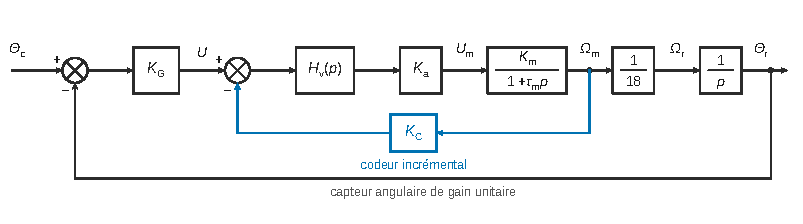
\includegraphics{figures/q31-schema-bloc.pdf}
\caption*{Figure 4 --- schéma de commande complété : boucle de vitesse interne
(codeur K\_C) et boucle de position à retour unitaire}
\end{figure}

\begin{piege}

Le réducteur donne une vitesse : il faut un intégrateur \(1/p\) pour passer de \(\Omega_r\) à \(\Theta_r\). Le retour de position n'a pas de bloc, puisque le capteur a un gain unitaire.

\end{piege}

\begin{jury}

Pour II.3, le rapport 2026 (p.~7) note que « Les questions classiques d'identification et de simplification de schémas-blocs sont globalement mieux réussies. » Q31 est réussie par environ 60 \% des candidats et Q32 par 74 \% (figure 2d, p.~5).

\end{jury}

\hypertarget{question-32}{%
\subsection{Question 32}\label{question-32}}

\begin{indication}{1}

Appliquer la formule de Black à la boucle interne, puis mettre le résultat sous forme canonique \(K/(1+\tau p)\).

\end{indication}

\hypertarget{solution-31}{%
\subsubsection{Solution}\label{solution-31}}

Chaîne directe de la boucle interne : \(K_vK_a\dfrac{K_m}{1+\tau_mp}\), retour \(K_C\). D'après la formule de Black,

\equationajustee{\begin{aligned}
H_1(p)&=\frac{K_vK_a\dfrac{K_m}{1+\tau_mp}}{1+K_CK_vK_a\dfrac{K_m}{1+\tau_mp}}\\
&=\frac{K_vK_aK_m}{1+K_CK_vK_aK_m+\tau_mp}\\
&=\frac{K_1}{1+\tau_1p},
\end{aligned}}

avec

\equationajustee{\boxed{\begin{aligned}
K_1&=\frac{K_vK_aK_m}{1+K_CK_vK_aK_m}\\
\tau_1&=\frac{\tau_m}{1+K_CK_vK_aK_m}
\end{aligned}}}

C'est un premier ordre, plus rapide que le moteur seul (\(\tau_1<\tau_m\)).

\begin{methode}

Une boucle de retour sur un premier ordre donne un premier ordre : le gain et la constante de temps sont tous deux divisés par \(1+K_{\text{boucle}}\).

\end{methode}

\hypertarget{question-33}{%
\subsection{Question 33}\label{question-33}}

\begin{indication}{1}

Appliquer le théorème de la valeur finale à \(\Omega_m\), puis comparer à la vitesse visée \(U_0/K_C\).

\end{indication}

\begin{indication}{2}

Transformer la condition en inégalité sur le gain de boucle \(K_CK_vK_aK_m\).

\end{indication}

\hypertarget{solution-32}{%
\subsubsection{Solution}\label{solution-32}}

Pour \(U=U_0/p\), le théorème de la valeur finale donne \(\Omega_m(\infty)=\lim_{p\to0}pH_1(p)\frac{U_0}{p}=K_1U_0\). La consigne de vitesse correspondant à \(U_0\) est \(U_0/K_C\) (vitesse pour laquelle le retour égale \(U_0\)). L'erreur statique vaut

\equationajustee{\begin{aligned}
\varepsilon_s&=\frac{U_0}{K_C}-K_1U_0\\
&=\frac{U_0}{K_C}\,\big(1-K_CK_1\big)\\
&=\frac{U_0}{K_C}\cdot\frac{1}{1+K_CK_vK_aK_m}.
\end{aligned}}

La condition \(\varepsilon_s<0{,}05\,\dfrac{U_0}{K_C}\) impose \(1+K_CK_vK_aK_m>20\), soit

\equationajustee{\boxed{K_v>\frac{19}{K_CK_aK_m}=\frac{19}{1\times1{,}3\times1{,}8}\approx8{,}1}}

(\(K_v\) est sans dimension.)

\begin{piege}

L'erreur relative se rapporte à la consigne de vitesse \(U_0/K_C\) et non à \(U_0\) : les unités ne sont pas les mêmes (\(\mathrm{rad\,s^{-1}}\) contre V).

\end{piege}

\begin{jury}

Q33 est la moins réussie de II.3, avec environ 12 \% de réussite (figure 2d, p.~5). Le rapport 2026 (p.~7) situe les difficultés dans « l'établissement analytique des fonctions de transfert et de l'étude de la précision des systèmes asservis ».

\end{jury}

\hypertarget{question-34}{%
\subsection{Question 34}\label{question-34}}

\begin{indication}{1}

Un correcteur agit sur un écart : où l'écart de position est-il disponible sous forme électrique ?

\end{indication}

\hypertarget{solution-33}{%
\subsubsection{Solution}\label{solution-33}}

Le correcteur \(C(p)\) agit sur l'écart de position. On l'insère dans la chaîne directe de la boucle de position, \textbf{entre le gain \(K_G\) du comparateur (sortie : écart en volts) et le comparateur de la boucle de vitesse} :

\begin{figure}[H]
\centering
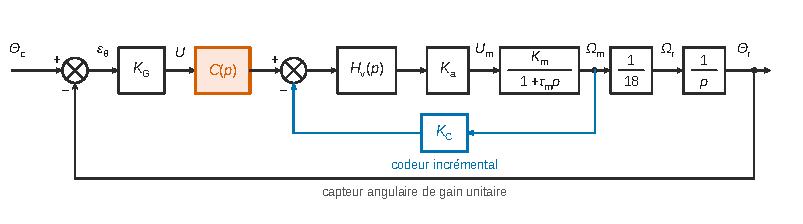
\includegraphics{figures/q34-schema-bloc-correcteur.pdf}
\caption*{Figure 5 --- schéma de commande avec le correcteur C(p) inséré entre
K\_G et la boucle de vitesse}
\end{figure}

Le correcteur se trouve ainsi en amont de la boucle de vitesse et hors de celle-ci.

\hypertarget{question-35}{%
\subsection{Question 35}\label{question-35}}

\begin{indication}{1}

Réduire la boucle interne à \(H_1\), puis multiplier les fonctions de transfert de la chaîne directe de position (retour unitaire).

\end{indication}

\begin{indication}{2}

Ordre = degré du dénominateur, classe = nombre d'intégrateurs.

\end{indication}

\hypertarget{solution-34}{%
\subsubsection{Solution}\label{solution-34}}

Avec \(C(p)=K_p\) et la boucle interne réduite à \(H_1(p)\), la fonction de transfert en boucle ouverte est \(\mathrm{FTBO}(p)=\Theta_r/\varepsilon_\theta\) :

\equationajustee{\begin{aligned}
\mathrm{FTBO}(p)&=K_G\,K_p\,H_1(p)\,\frac1{18}\,\frac1p\\
&=\boxed{\frac{K_{BO}}{p\,(1+\tau_1p)}},
\end{aligned}}

avec

\equationajustee{\boxed{K_{BO}=\frac{K_GK_pK_1}{18}}}

Le dénominateur est de degré 2, donc \textbf{ordre 2}. Il y a un pôle nul simple (intégrateur), donc \textbf{classe 1}.

\begin{piege}

La FTBO de la boucle de position se calcule avec la boucle de vitesse déjà fermée, remplacée par \(H_1\) ; seule la boucle de position est ouverte. L'ordre est le degré du dénominateur, la classe le nombre d'intégrateurs : ici 2 et 1.

\end{piege}

\begin{jury}

Le rapport 2026 (p.~7) attribue les erreurs de II.3 à « la manipulation des boucles imbriquées, de la distinction entre boucle ouverte et boucle fermée, et des notions d'ordre, de classe et d'erreur statique ». Q35 est réussie par environ 18 \% des candidats (figure 2d, p.~5).

\end{jury}

\hypertarget{question-36}{%
\subsection{Question 36}\label{question-36}}

\begin{indication}{1}

Écrire l'écart en fonction de la consigne et de la FTBO, puis appliquer le théorème de la valeur finale à un échelon.

\end{indication}

\hypertarget{solution-35}{%
\subsubsection{Solution}\label{solution-35}}

Le retour est unitaire, donc l'écart \(\varepsilon_\theta=\Theta_c-\Theta_r\) s'écrit \(\varepsilon_\theta(p)=\dfrac{\Theta_c(p)}{1+\mathrm{FTBO}(p)}\). Pour un échelon \(\Theta_c=\theta_0/p\), le théorème de la valeur finale donne

\equationajustee{\begin{aligned}
\varepsilon_s&=\lim_{p\to0}p\,\frac{\theta_0/p}{1+\dfrac{K_{BO}}{p(1+\tau_1p)}}\\
&=\lim_{p\to0}\frac{\theta_0\,p(1+\tau_1p)}{p(1+\tau_1p)+K_{BO}}\\
&=\boxed{0}
\end{aligned}}

\textbf{L'erreur statique de position est nulle}, grâce à l'intégrateur en boucle ouverte (classe 1). Le système en boucle fermée est un second ordre à coefficients positifs, donc stable.

\begin{methode}

Avec un retour unitaire, une FTBO de classe \(n\) donne une erreur nulle pour toute consigne polynomiale de degré inférieur à \(n\), une erreur finie pour le degré \(n\), et une erreur infinie au-delà.

\end{methode}

\hypertarget{question-37}{%
\subsection{Question 37}\label{question-37}}

\begin{indication}{1}

Même calcul avec une rampe \(a/p^2\) : le résultat est-il nul, fini ou infini pour une classe 1 ?

\end{indication}

\begin{indication}{2}

Pour corriger, il faut augmenter la classe ; vérifier alors la stabilité (critère de Routh sur un polynôme de degré 3).

\end{indication}

\hypertarget{solution-36}{%
\subsubsection{Solution}\label{solution-36}}

Pour une rampe \(\Theta_c=a/p^2\) :

\equationajustee{\begin{aligned}
\varepsilon_v&=\lim_{p\to0}p\,\frac{a/p^2}{1+\dfrac{K_{BO}}{p(1+\tau_1p)}}\\
&=\frac{a}{K_{BO}}\\
&=\frac{18\,a}{K_GK_pK_1}\neq0 .
\end{aligned}}

\textbf{L'erreur de traînage est finie mais non nulle.} Pour l'annuler, il faut une FTBO de classe 2, donc un second intégrateur, placé dans le correcteur. On choisit un \textbf{correcteur à action intégrale de type PI}, \(C(p)=K_p\dfrac{1+T_ip}{T_ip}\), plutôt qu'un intégrateur pur.

Avec un intégrateur pur, la FTBO \(\frac{K}{p^2(1+\tau_1p)}\) donnerait un système bouclé instable. Avec le PI, l'équation caractéristique \(T_i\tau_1p^3+T_ip^2+K_{BO}T_ip+K_{BO}=0\) est stable si et seulement si \(T_i>\tau_1\) (critère de Routh). Le zéro du PI apporte l'avance de phase nécessaire.

\begin{piege}

Un intégrateur pur ajouté à une FTBO de classe 1 d'ordre 2 rend le système bouclé instable. Le zéro du PI est indispensable. Il ne suffit pas d'écrire « ajouter un intégrateur ».

\end{piege}

\begin{jury}

Selon le rapport 2026 (p.~7), « La très forte participation à la dernière question confirme enfin que les candidats ont correctement identifié son caractère accessible et relativement indépendant des calculs précédents. » Les histogrammes numérotent cette dernière question « Q38 » (abordée par presque tous, réussie par environ 63 \%), alors que le sujet s'arrête à Q37. La correspondance exacte entre les items Q36 à Q38 du rapport et les questions 36 et 37 du sujet n'est pas précisée.

\end{jury}

\hypertarget{bilan}{%
\section{Bilan}\label{bilan}}

\textbf{Méthodes à retenir.}

\begin{itemize}
\tightlist
\item
  \emph{Plasma froid} : principe fondamental, force magnétique négligée (ordre \(v/c\)), ions négligés (ordre \(m_e/m_i\)). On en tire \(\underline\sigma=\mathrm i n e^2/(m\omega)\) puis \(k^2c^2=\omega^2-\omega_p^2\). Le même enchaînement sert pour les métaux (modèle de Drude) et pour la réflexion ionosphérique.
\item
  \emph{Dispersion} : \(v_\varphi=\omega/k\) et \(v_g=\mathrm d\omega/\mathrm dk\). Un milieu est dispersif si \(v_\varphi\) dépend de \(\omega\). Un signal de largeur spectrale non nulle s'étale.
\item
  \emph{Référentiel tournant} : forces d'entraînement et de Coriolis. La force centrifuge dérive d'une énergie potentielle \(-\frac12m\Omega^2r^2\), la force de Coriolis ne travaille pas : on obtient une intégrale première (Jacobi) et des régions accessibles \(U\ge C_J/2\).
\item
  \emph{Équilibres et stabilité} : on annule le gradient en tenant compte des dérivées composées, on linéarise, on écrit le système d'état \(\dot{\mathbf Y}=\mathbf A\mathbf Y\), puis on discute les valeurs propres. Stabilité (au sens d'un mouvement borné) si toutes les valeurs propres sont imaginaires pures et simples.
\item
  \emph{Dynamique des systèmes de solides} : choisir pour chaque équation un système isolé et un point qui éliminent les inconnues de liaison (point sur l'axe d'une pivot parfaite). Utiliser le transport \(\vec\delta_A=\vec\delta_G+\overrightarrow{AG}\wedge m\vec a_G\) et les actions réciproques.
\item
  \emph{Asservissements} : formule de Black, théorème de la valeur finale, lien classe--précision (classe 1 : erreur nulle en échelon, finie en rampe), correcteur PI et sa condition de stabilité.
\end{itemize}

\textbf{Questions discriminantes (rapport 2026).} La partie I.2 entière (15 \% de réussite globale), en particulier Q7.b, Q8, Q10--Q11 et Q13--Q17 ; en SI, Q21--Q22 et Q25--Q28 ; en automatique, Q33 et Q35. Le rapport (p.~7) résume les pertes de points en trois natures : « difficultés de modélisation, erreurs dans les développements calculatoires et insuffisance des justifications physiques ». Il y ajoute les applications numériques, les unités et les items oubliés.

\textbf{Prérequis à revoir.} Notation complexe et opérateur \(\vec\nabla\to\mathrm i\vec k\), double produit vectoriel, moments d'inertie usuels (tige, plaque, parallélépipède), dérivation vectorielle dans une base mobile, théorème de la valeur finale.

\textbf{Questions classiques transposables.}

\begin{itemize}
\tightlist
\item
  Pulsation plasma et coupure ionosphérique : se retrouve dans les sujets sur les métaux, les ondes radio et la réflexion totale.
\item
  Troisième loi de Kepler et constante de Jacobi : se retrouvent dans les sujets sur les satellites, les marées et les points de Lagrange.
\item
  Linéarisation et critère de stabilité par valeurs propres : se retrouve pour le pendule, le gyroscope ou l'équilibre d'un satellite.
\item
  Équations du mouvement d'un double pendule plan : c'est exactement la structure de Q26--Q27.
\item
  Boucle de vitesse interne puis boucle de position : c'est le schéma standard de tous les sujets d'asservissement de moteurs.
\end{itemize}

\end{document}
